%%%% utfpr-slides.tex, 2019/12/01
%%%% Copyright (C) 2015-2019 Luiz E. M. Lima (luizeduardomlima@gmail.com)
%%
%% This work may be distributed and/or modified under the conditions of the
%% LaTeX Project Public License, either version 1.3 of this license or (at your
%% option) any later version.
%% The latest version of this license is in
%%   http://www.latex-project.org/lppl.txt
%% and version 1.3 or later is part of all distributions of LaTeX version
%% 2005/12/01 or later.
%%
%% This work has the LPPL maintenance status `maintained'.
%%
%% The Current Maintainer of this work is Luiz E. M. Lima.
%%
%% This work consists of the files utfpr-slides.sty and utfpr-slides.tex.
%%
%% A brief description of this work is in readme.txt.

%% Detecção e aviso sobre comandos obsoletos
% \RequirePackage[l2tabu, orthodox]{nag}

%% Classe de documento e opções
%%%% Modo apresentação: descomente o comando \documentclass[]{beamer}
\documentclass[%% Opções: [*] comente para remover; [>] passada para pacotes
  10pt,%% Tamanho de fonte: 10pt, 11pt, 12pt, etc.
  aspectratio = 169,%% Razão de aspecto: 169 (16:9), 43 (4:3), etc.
  compress,%% Redução de tamanho das barras de navegação [*]
  % handout,%% Versão que usa especificações de sobreposição do folheto [*]
  t,%% Alinhamento vertical dos quadros: b (fundo), c (centro) e t (topo)
  english,%% Idioma secundário (penúltimo) [>]
  brazilian,%% Idioma primário (último) [>]
  tikz,
]{beamer}
%%%% Modo artigo: descomente o comando \documentclass[]{article}
% \documentclass[%% Opções: [>] passada para pacotes
  % a4paper,%% Tamanho de papel: a4paper, letterpaper, etc.
  % english,%% Idioma secundário (penúltimo) [>]
  % brazilian,%% Idioma primário (último) [>]
% ]{article}
% \documentclass[tikz]{article}

%% Pacotes utilizados
\usepackage[%% Opções:
  Times   = false,%% Fontes Times (roman) e Arial (sans serif): true ou false
  BibURLs = false,%% Links de URLs nas referências: true ou false
  GovLogo = false,%% Logomarca do Governo Federal: true ou false
  MECLogo = false,%% Logomarca do Ministério da Educação: true ou false
  LogosOn = false,%% Logomarcas nos títulos dos slides: true ou false
  ABNTNum = none,%% Estilo numérico ABNT: none (AUTOR, ANO), dflt (1) e brkt [1]
]{utfpr-slides}
\usepackage{color,soul}
\sethlcolor{yellow}
\usepackage{multirow}

%% Arquivo de referências
\addbibresource{utfpr-slides.bib}

%% Arquivos de logomarcas (diretório ``Logos''): comente para remover
\logoevent{evento}%% Logomarca do evento
\logoorg{evento-org}%% Logomarca da organização promotora
\logoextinst{inst-ext}%% Logomarca da instituição do autor externo
\logoprog{ppgcc-pg}%% Logomarca do programa ou do curso
% \logodept{depto}%% Logomarca do departamento ou da coordenação
\logoextra{utfpr-110anos}%% Logomarca extra (à esquerda da logomarca do câmpus)
\logocampus{utfpr-pg}%% Logomarca do câmpus

%% Informações do documento
%%%% Título: [CURTO]; {LONGO}
\title[REDES NEURAIS CONVOLUCIONAIS NA SEGMENTAÇÃO SEMÂNTICA DE IMAGENS AÉREAS PARA O MAPEAMENTO DA COBERTURA DA TERRA EM ÁREAS DE PROTEÇÃO AMBIENTAL]{%
  \bfseries%
  Redes Neurais Convolucionais na Segmentação Semântica
  \\de Imagens Aéreas para o Mapeamento da Cobertura da Terra
  \\em Áreas de Proteção Ambiental
  % Título da Apresentação em Congresso, Seminário ou Evento%
  % \\Técnico/Científico, ou para Defesa de Trabalho Acadêmico%
}
%%%% Subtítulo
% \subtitle{%
%   Subtítulo da Apresentação em Congresso, Seminário ou Evento%
%   \\Técnico/Científico, ou para Defesa de Trabalho Acadêmico%
% }
%%%% Assunto
\subject{Nome e/ou Sigla do Congresso, Seminário ou Evento Técnico/Científico}
%%%% Congresso, seminário ou evento técnico/científico:
%%%% descomente os comandos \author[]{}, institute[]{} e \titlegraphic{}
%%%%%% Autor(es): [CURTO]; {LONGO}
\author[P. M. Autor(a) et al.]{%
  Fabricio Bizotto\inst{1}%
  \athanks[0000-0000-0000-0001]{fabriciobizotto@alunos.utfpr.edu.br}{%
    Departamento, Coordenação, Programa ou Curso%
  }%
  \and Mauren L Andrade\inst{2}%
  \athanks[0000-0000-0000-0002]{autor2@dominio}{%
    Departamento, Coordenação, Programa ou Curso%
  }%
  \and Gilson A Giraldi\inst{3}%
  \athanks[0000-0000-0000-0003]{autor3@dominio}{%
    Departamento, Coordenação, Programa ou Curso%
  }%
  }
%%%%%% Instituição(ões) e e-mail(s): [CURTO]; {LONGO}
\institute[UTFPR/INST-EXT]{%
  \affil[1,2]{\utfprname, Ponta Grossa, Paraná, Brasil}%
  \and\affil[3]{Departmento de Engenharia Elétrica, Pontifícia Universidade Católica do Rio de Janeiro, RJ, Brazil}%
  \and\email[1]{fabriciobizotto@alunos.utfpr.edu.br}%
  \sep\email[2]{autor2@dominio}%
  \sep\email[3]{autor3@dominio}%
  \sep\email[4]{autor4@dominio}%
  \sep\email[5]{autor5@dominio}%
}
%%%%%% Logomarcas do evento
\titlegraphic{\eventlogos}
%%%% Defesa de trabalho acadêmico:
%%%% descomente os comandos \author[]{}, institute[]{} e \titlegraphic{}
%%%%% Autor(a): [CURTO]; {LONGO}
\author[Fabricio]{%
  Fabricio Bizotto%
  \athanks[0000-0000-0000-0000]{fabriciobizotto@alunos.utfpr.edu.br}{%
    Programa de Pós-Graduação em Ciência da Computação%
  }%
}
%%%%% Instituição: [CURTO]; {LONGO}
\institute[UTFPR-PG/DAINF/PPGCC]{%
  \affil{%
    \utfprname\ (UTFPR)%
    \and Câmpus Ponta Grossa (PG)%
    \and Departamento Acadêmico de Informática (DAINF)%
    \and Programa de Pós-Graduação em Ciência da Computação (PPG-CC)%
  }%
  \and\email{mlsguario@utfpr.edu.br}%
  \and Orientadora: Profa. Dra. Mauren L Andrade%
}
%%%%% Logomarcas da instituição
\titlegraphic{\institutelogos}
%%%% Câmpus: {SIGLA}; {NOME}
\campus{PG}{Câmpus Ponta Grossa}
%%%% Departamento, coordenação, programa ou curso: [LOGO]; {SIGLA}; {NOME}
\departament[depto]{DEPTO}{Departamento, Coordenação, Programa ou Curso}
%%%% Data: [CURTO]; {LONGO}
% \date[\today]
\date[21 de novembro de 2023]

%% Início do documento
\begin{document}

\mode<presentation>{%% Modo apresentação: página de título e sumário
  \frame{\titlepage}%
  \frame[allowframebreaks]{%
    \frametitle{\contentsname}%
    \framesubtitle{~}%
    \tableofcontents%
  }%
}

\mode<article>{\maketitle}%% Modo artigo: página de título

\section{Introdução}\label{sec:intro}

\begin{frame}{Introdução}
    \begin{itemize}
        \item Área de Proteção Ambiental (APA)
        \begin{itemize}
            \item Ferramenta de Conservação da Natureza.
            \item Destinada à proteção ambiental e ao uso sustentável dos recursos naturais.
            \item Objetivo: Conservação x Desenvolvimento Econômico.
            \item Gestão governamental, como o Instituto Chico Mendes de Conservação da Biodiversidade (ICMBio).
            \item Regulamenta as atividades humanas de acordo com as características ambientais da região.
        \end{itemize}
    \end{itemize}
    \begin{block}{Principais desafios no monitoramento da APA}
        \begin{itemize}
            \item Grandes equipes de trabalho especializada
            \item Deslocamento à regiões de difícil acesso
            \item Alto custo para manutenção das equipes
            \item Perigos associados as características de fauna e flora de cada região
        \end{itemize}
    \end{block}
\end{frame}

% \begin{frame}
% \begin{columns}[T]

% \column{0.5\textwidth}
% A Fig.~\ref{fig:apa} representa a área da APA-Petrópolis, região serrana do Rio de Janeiro.
% \begin{figure}[!htb]
% \centering%
% \caption{APA-Petrópolis.}%
% % \label{fig:apa}
% \mode<presentation>{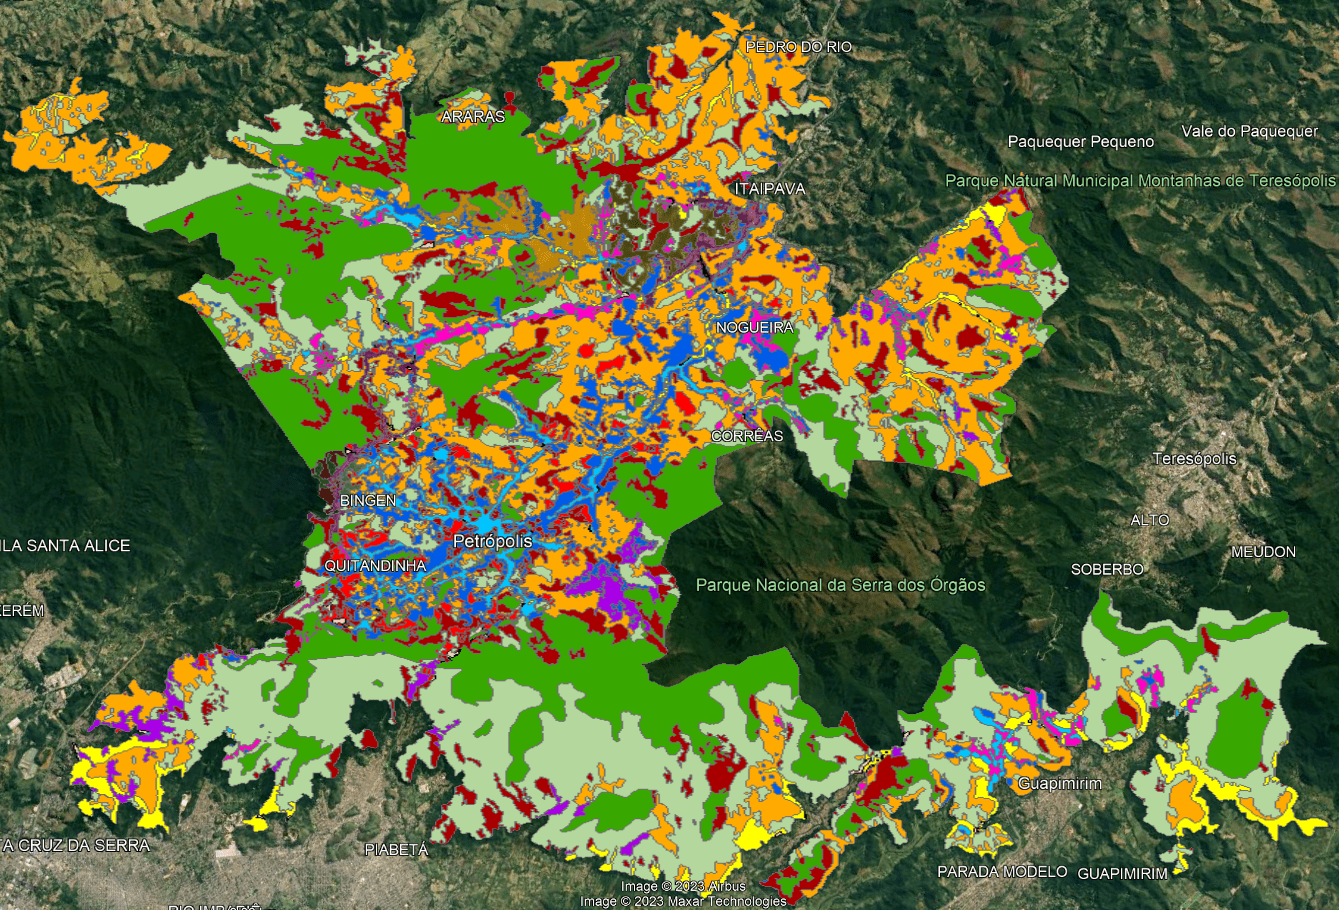
\includegraphics[width = 0.8\columnwidth]{./Figuras/apa}}%% Modo apresentação: tamanho da figura
% \mode<article>{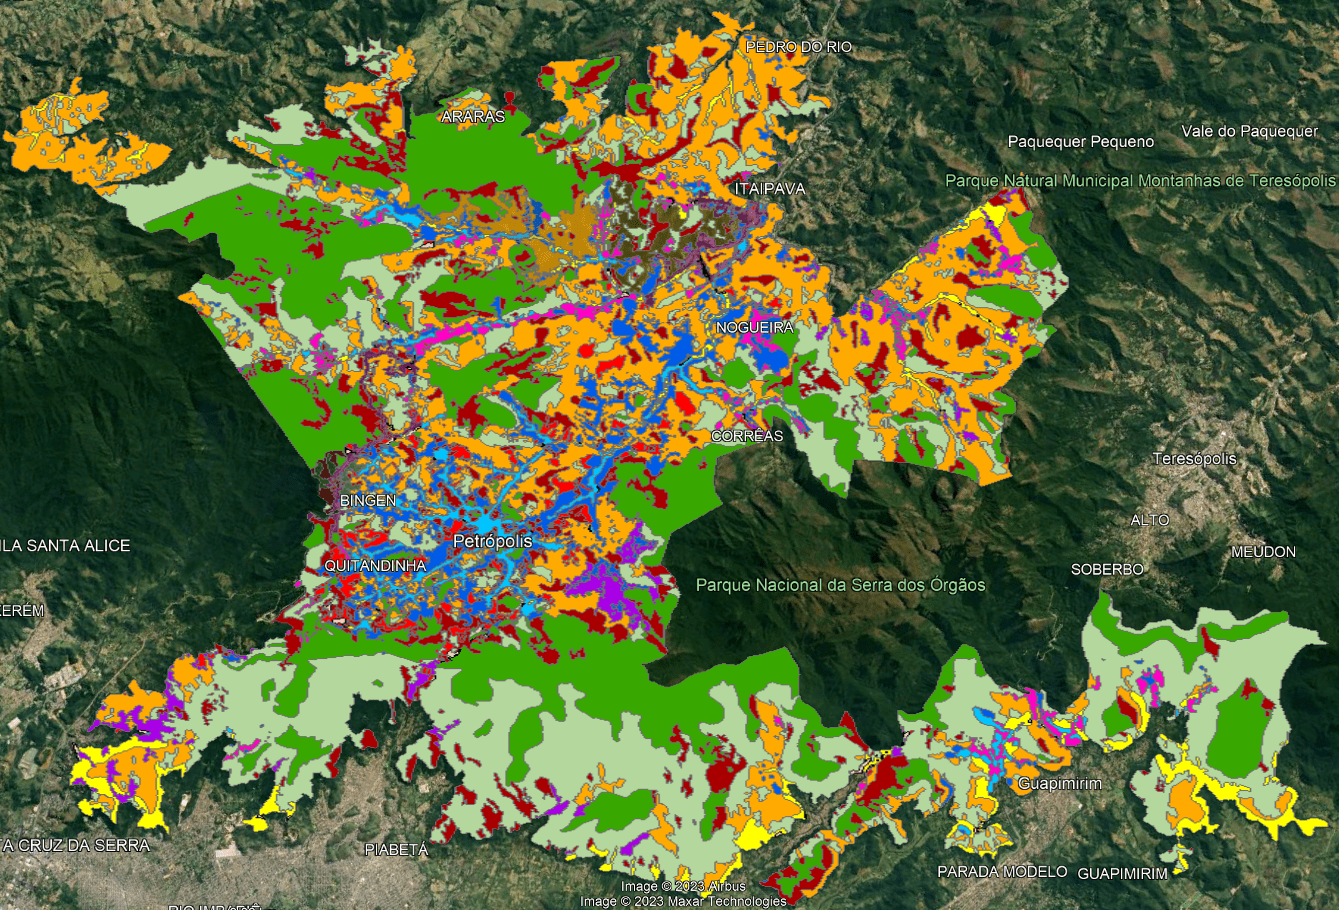
\includegraphics[width = 0.4\columnwidth]{./Figuras/apa}}%% Modo artigo: tamanho da figura
% \source{\cite{GE2023}.}
% \end{figure}
% \column{0.5\textwidth}
% \mode<article>{\par}%% Modo artigo: quebra de parágrafo
% \begin{block}{APA-Petrópolis}
% \begin{itemize}
% \item $\approx$ 60.000 hectares
% \item Ações de conservação realizadas pelo ICMBio:
% \begin{itemize}
%     \item Monitoramento Ambiental
%     \item Manutenção de trilhas ecológicas
%     \item Recuperação de áreas degradadas
%     \item Combate a incêndios
%     \item Proteção de espécies ameaçadas de extinção
%     \item Invasão de terras
% \end{itemize}
% \end{itemize}
% \end{block}
% \end{columns}
% \end{frame}

% \begin{frame}{Introdução}
% \begin{itemize}
%     \item A cobertura e utilização do solo \textbf{(Land Use and Land Cover - LULC)}
%     % \item O desenvolvimento socioeconômico dos seres humanos tem sido fortemente apoiado pelo uso da terra, sendo a urbanização um dos principais exemplos de mudanças de ocupação do solo em todo o mundo \cite{LIU, 2018}.
%     \item Compreender a relação entre cobertura e uso da terra é essencial para gerir os recursos naturais, mitigar as alterações climáticas e proteger a biodiversidade \cite{ZIN; LIN, 2018}.
%     \item Mudanças antropogênicas abrangem o desflorestamento, desocupação, urbanização, alterações nos tipos de cultivo e adaptações nas práticas utilizadas em cada uso do solo, tais como, técnicas de plantio e sistemas de rotação de cultura florestal \cite{Peterson et al. (2014)}.
%     % \begin{block}{Principais desafios no monitoramento da APA}
%     %     \begin{itemize}
%     %         \item Grandes equipes de trabalho especializada
%     %         \item Deslocamento à regiões de difícil acesso
%     %         \item Alto custo para manutenção das equipes
%     %         \item Perigos associados as características de fauna e flora de cada região
%     %     \end{itemize}
%     % \end{block}
% \end{itemize}
% \end{frame}

\begin{frame}{Introdução}

\textbf{Sensoriamento Remoto}

    \begin{itemize}
        \item Alternativa de baixo custo
        \item Acesso a base de dados de imagens para diferentes regiões
        \item Acesso a áreas de difícil acesso via solo
        \item Estudos começam a exploraram a aplicação das Redes Neurais Convolucionais (RNC) na análise da cobertura da terra com resultados promissores \cite{HU et al., 2013), (LI et al., 2020}.
    \end{itemize}

    % \begin{block}{Possibilidades}
    %     \begin{itemize}
    %         \item Imagens de satélite disponíveis gratuitamente
    %         \item VANT (Veículo Aéreo não Tripulado) (custo alto)
    %         \item Imagens Aéreas RGB da plataforma Google Earth
    %     \end{itemize}
    % \end{block}

\end{frame}



\subsection{Objetivo Geral}\label{ssec:intro1}

\begin{frame}
O objetivo geral deste trabalho é o desenvolvimento de uma nova metodologia para segmentação semântica de imagens de sensoriamento remoto do Google a fim de gerar o mapa de cobertura e uso do solo da região da APA-Petrópolis, Rio de Janeiro por meio de RNC
% Esta apresentação de slides foi desenvolvida com base na classe \href{http://www.ctan.org/pkg/beamer/}{\LaTeX/Beamer~\linkicon}.
% \begin{block}{Citações e referências}
% \begin{itemize}
% \item Exemplos de referências podem ser observados nas citações:
% \begin{itemize}
% \item Implícita: \ldots\ \cite{Nriagu1988,Lamport1994,VanEkenstein1997}.
% \item Explícita: Segundo \textcite{Wizentier1992,Faina2000},\ldots
% \end{itemize}
% \item Citações e referências podem ser inseridas neste documento usando os comandos do pacote \LaTeX\ \enquote{\href{http://ctan.org/pkg/biblatex/}{biblatex~\linkicon}}.
% \item Os dados de cada referência podem ser obtidos de um arquivo \enquote{bibtex} (*.bib), geralmente na própria página de \textit{download} da referência (artigos, livros, etc.), ou no Google Acadêmico, etc.
% \item Para gerar ou editar entradas de arquivos \enquote{bibtex} (*.bib), pode-se utilizar a ferramenta \enquote{\href{http://truben.no/latex/bibtex/}{Bibtex Editor~\linkicon}} ou \enquote{\href{http://zbib.org/}{ZoteroBib~\linkicon}}, entre outras.
% \end{itemize}
% \end{block}
\end{frame}

\subsection{Objetivos Específicos}\label{sec:intro2}

\begin{frame}
Para atender o objetivo geral deste trabalho, foram propostos os seguintes objetivos específicos:

\begin{block}<+->{Objetivos Específicos}
\begin{itemize}
\item Capturar e rotular imagens de sensoriamento remoto da área de proteção ambiental de
Petrópolis, Rio de Janeiro.
\item Comparar o desempenho de redes neurais do tipo SegNet e U-NET no conjunto de dados criado.
\item Comparar diferentes funções de custo a fim de avaliar a que melhor se adapte ao conjunto
de dados.
\item Utilizar métricas para analisar e comparar o desempenho dos modelos.
\item Comparar os resultados obtidos com trabalhos relacionados.
\end{itemize}
\end{block}
\end{frame}

\subsection{Trabalhos Relacionados}\label{sec:intro3}

\begin{frame}
    % 1. Construção de mapas digitais a partir de imagens de satélite, utilizando a arquitetura U-Net com EfficientNet-B0 como codificador e decodificador \textbf{\cite{Khanh2021}}.
    1.  Construção de mapas digitais a partir de imagens aéreas do Google, usando a arquitetura EfficientNet-B0 como codificador para extrair as características geográficas e U-Net como decodificador para reconstruir o mapa de características\textbf{\cite{Khanh2021}}.
    \begin{figure}[!htb]
        \centering%
        \caption{Resultado da segmentação semântica no conjunto de dados do Google com a arquitetura proposta.}%
        \label{fig:khan01}
        \mode<presentation>{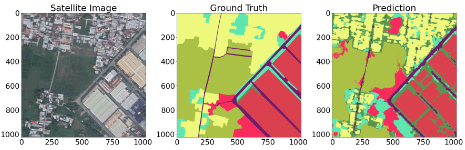
\includegraphics[width = 0.8\columnwidth]{./Figuras/khan-01}}%% Modo apresentação: tamanho da figura
        \mode<article>{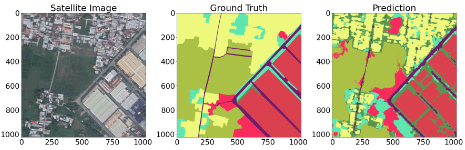
\includegraphics[width = 0.4\columnwidth]{./Figuras/khan-01}}%% Modo artigo: tamanho da figura
        \source{Adaptado de \cite{Khanh2021}.}
    \end{figure}
    
\end{frame}

% \begin{frame}
%     2. Aplicação de RNC, na tarefa de segmentação semântica de imagens obtidas por sensoriamento remoto. Duas arquiteturas de RNC, SegNet e U-net, são aprimoradas por meio da introdução de \textit{index pooling} para melhorar essas arquiteturas, permitindo a preservação de informações espaciais cruciais durante a ampliação da resolução. \textbf{\cite{Alam2021}}.
%     \begin{figure}[!htb]
%         \centering%
%         \caption{Resultado da segmentação semântica.}%
%         \label{fig:alam2021}
%         \mode<presentation>{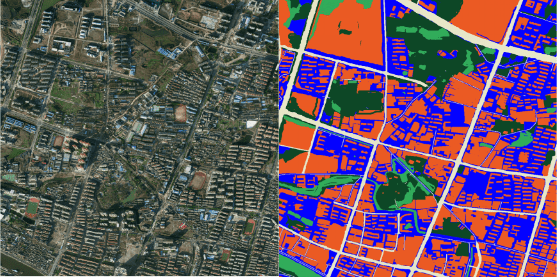
\includegraphics[width = 0.6\columnwidth]{./Figuras/Alam2021}}%% Modo apresentação: tamanho da figura
%         \mode<article>{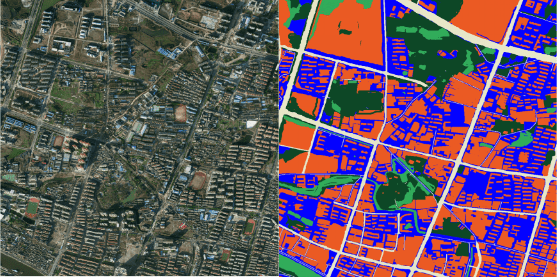
\includegraphics[width = 0.4\columnwidth]{./Figuras/Alam2021}}%% Modo artigo: tamanho da figura
%         \source{Adaptado de \cite{Alam2021}.}
%     \end{figure}
    
% \end{frame}

% \begin{frame}
%     3. Arquitetura U-Net para segmentar estufas agrícolas de plástico em imagens de sensoriamento remoto de alta resolução. A abordagem foi dividida em três etapas: coleta e anotação de imagens, treinamento da rede U-Net e pós-processamento para remover elementos confundíveis com as estufas \textbf{\cite{Chen2021}}.
%     \begin{figure}[!htb]
%         \centering%
%         \caption{Dificuldade em extrair estufas densamente distribuidas.}%
%         \label{fig:alam2021}
%         \mode<presentation>{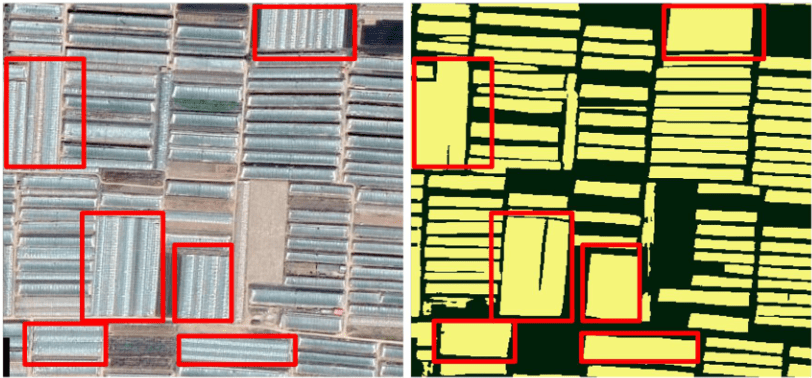
\includegraphics[width = 0.6\columnwidth]{./Figuras/apg}}%% Modo apresentação: tamanho da figura
%         \mode<article>{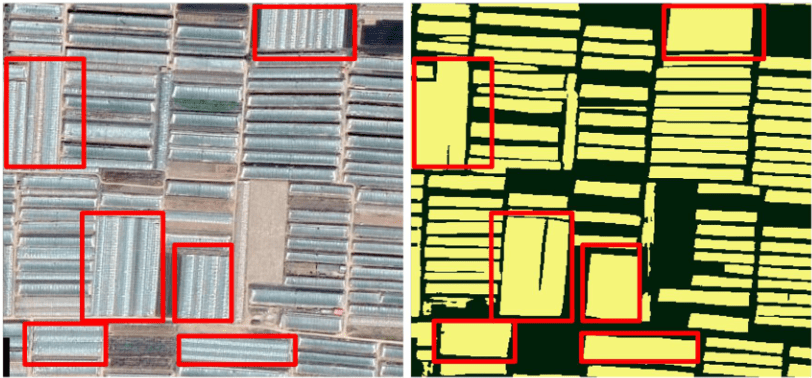
\includegraphics[width = 0.4\columnwidth]{./Figuras/apg}}%% Modo artigo: tamanho da figura
%         \source{\cite{Chen2021}.}
%     \end{figure}
    
% \end{frame}

% \section{Revisão da Literatura}\label{sec:revlit}

% \subsection{Processamento Digital de Imagem}\label{ssec:revlit1}

% \begin{frame}
% % \begin{block}<+->{Formação da Imagem Digital}
% \begin{itemize}
% \item Amostragem: Resolução espacial.
% \item Quantização: Intensidade de brilho.
% \end{itemize}
% % \end{block}

% \begin{figure}[!htb]
%     \centering%
%     \caption{Imagem projetada em uma matriz bidimensional.}%
%     \label{fig:alam2021}
%     \mode<presentation>{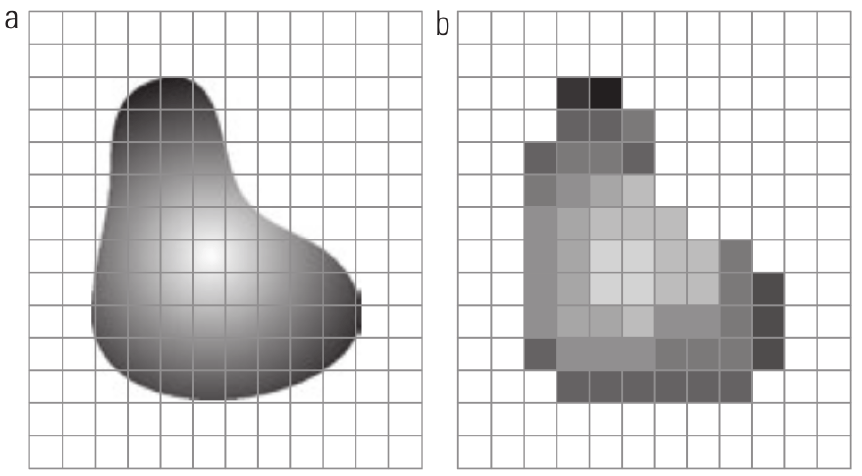
\includegraphics[width = 0.5\columnwidth]{./Figuras/amo_qua}}%% Modo apresentação: tamanho da figura
%     \mode<article>{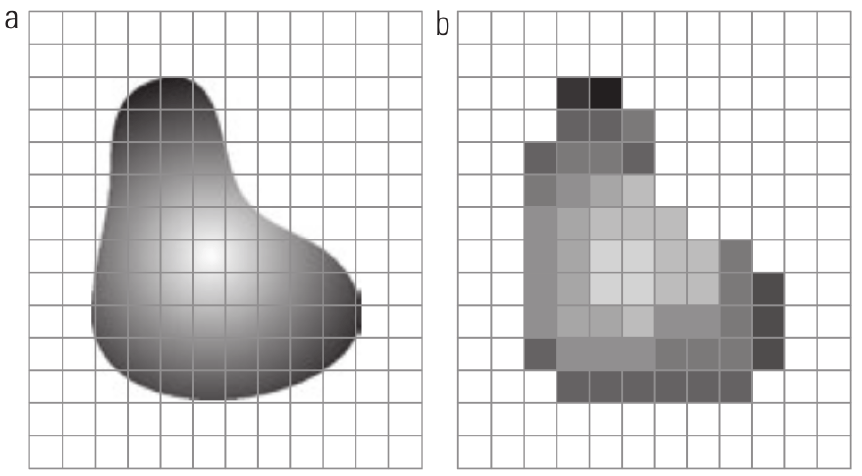
\includegraphics[width = 0.4\columnwidth]{./Figuras/amo_qua}}%% Modo artigo: tamanho da figura
%     \source{\cite{Gonzalez2009}.}
% \end{figure}
% \end{frame}

% \subsection{Equações, com e sem Numeração}\label{ssec:revlit2}

% \begin{frame}[fragile = singleslide]
% Uma equação como $y = a x^2 + b x + c$ pode ser inserida ao longo do texto de um parágrafo usando o ambiente \LaTeX\ \enquote{math} (\verb|$...$|).
% Por outro lado, a seguinte equação é um exemplo de equação não numerada inserida numa linha em separado usando o ambiente \LaTeX\ \enquote{displaymath} (\verb|\[...\]|).
% \begin{block}{}
% \[
% \frac{\mathrm{d} y}{\mathrm{d} x} = \gamma \operatorname{sen} x
% \]
% \end{block}
% A Eq.~\eqref{eq:fx} é um exemplo de equação inserida usando o ambiente \LaTeX\ \enquote{equation} e numerada automaticamente.
% \begin{block}{}
% \begin{equation}\label{eq:fx}
% f(x) = \frac{1}{\alpha} \int_0^L \left(\frac{x^2}{2} - \frac{x^3}{3}\right) \mathrm{d} x
% \end{equation}
% \end{block}
% Para gerar ou editar equações em \LaTeX, pode-se utilizar a ferramenta \enquote{\href{http://formulasheet.com/}{Formula Sheet~\linkicon}}, entre outras.
% \end{frame}

\section{Material e Métodos}\label{sec:matmet}

\subsection{Metodologia Proposta}\label{ssec:matmet1}

\begin{frame}
A Fig.~\ref{fig:metodologia} apresenta a metodologia utilizada para a realização dos objetivos propostos.
\begin{figure}[!htb]
\centering%
\caption{Metodologia Proposta.}%
\label{fig:metodologia}
\mode<presentation>{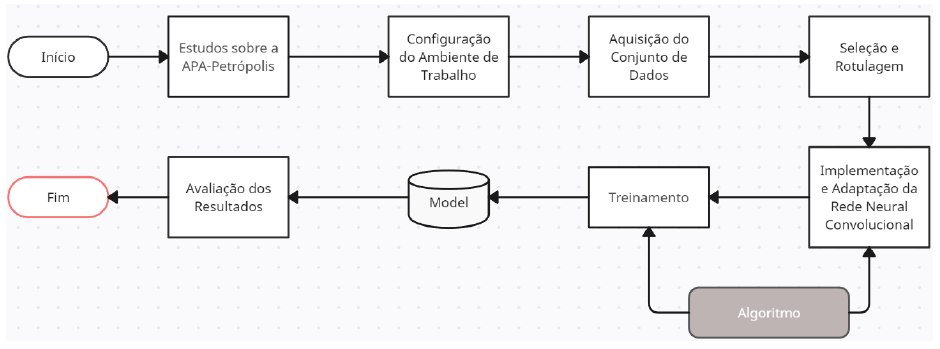
\includegraphics[width = 0.8\columnwidth]{./Figuras/metodologia}}%% Modo apresentação: tamanho da figura
\mode<article>{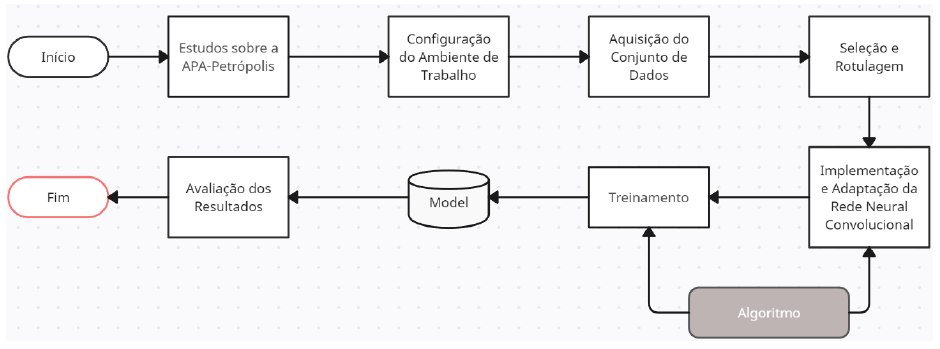
\includegraphics[width = 0.4\columnwidth]{./Figuras/metodologia}}%% Modo artigo: tamanho da figura
\source{Autoria Própria.}
\end{figure}
\end{frame}

\subsection{Estudos sobre a APA-Petrópolis}\label{ssec:matmet2}

\begin{frame}
\begin{columns}[T]

\column{0.5\textwidth}
% \begin{itemize}
%     \item $\approx$ 60.000 hectares (5,69\%) da Mata Atlântica.
%     \item Região urbanizada.
%     \item Plano de manejo que define ações e restrições.
%     \item Petrópolis e municípios adjacentes.
% \end{itemize}

\begin{itemize}
    \item $\approx$ 68.000 hectares.% (5,69\%) da Mata Atlântica.
    \item Região urbanizada.
    \item Plano de manejo que define ações e restrições.
    \item Petrópolis e municípios adjacentes.
    \item Ações de conservação realizadas pelo ICMBio:
    \begin{itemize}
        \item Monitoramento Ambiental
        \item Manutenção de trilhas ecológicas
        \item Recuperação de áreas degradadas
        \item Combate a incêndios
        \item Proteção de espécies ameaçadas de extinção
        \item Invasão de terras
    \end{itemize}
\end{itemize}

\column{0.5\textwidth}
A Fig.~\ref{fig:apa} representa a área da APA-Petrópolis, região serrana do Rio de Janeiro.
\begin{figure}[!htb]
\centering%
\caption{APA-Petrópolis.}%
\label{fig:apa}
\mode<presentation>{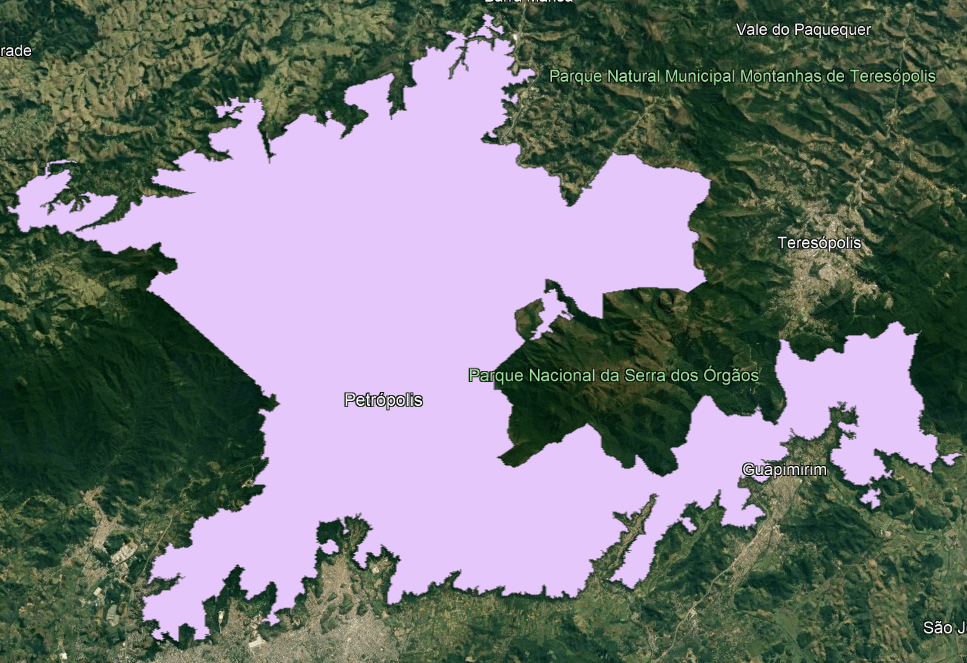
\includegraphics[width = 1.0\columnwidth]{./Figuras/apa-min}}%% Modo apresentação: tamanho da figura
\mode<article>{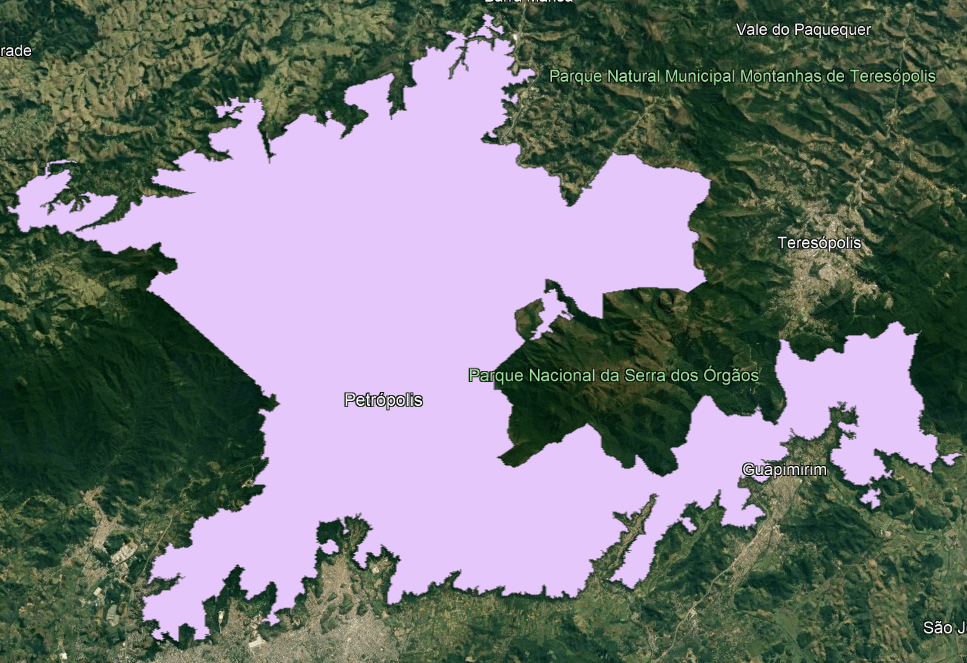
\includegraphics[width = 0.8\columnwidth]{./Figuras/apa-min}}%% Modo artigo: tamanho da figura
\source{Adaptado de \cite{GE2023}.}
\end{figure}
\end{columns}
\end{frame}

\subsection{Configuração do ambiente de Trabalho}\label{ssec:matmet3}

\begin{frame}
\begin{columns}[T]
\column{0.5\textwidth}
\begin{itemize}
    \item \textbf{Processador}: Intel(R) Xeon(R) CPU E5-2666 v3 @ 2.90GHz 2.90 GHz;
    \item \textbf{Memória RAM}: 32 GB;
    \item \textbf{Placa de Vídeo}: NVIDIA GIGABYTE RTX 3060 EAGLE OC – 12GB dedicada;
    \item \textbf{Sistema Operacional}: Microsoft Windows 10 PRO 64 bits.
\end{itemize}
\column{0.5\textwidth}

A Tab.~\ref{tab:tools} apresenta o conjunto de ferramentas utilizado durante o trabalho.
\begin{table}[!htb]
\centering%
\mode<presentation>{\scriptsize}%% Modo apresentação: tamanho de fonte
\mode<article>{\small}%% Modo artigo: tamanho de fonte
\caption{Conjunto de Ferramentas Utilizadas.}%
\label{tab:tools}
\begin{tabular*}{\columnwidth}{@{\extracolsep{\fill}}ll}
\toprule
Python                                   & \cite{PythonManual}           \\
PyTorch                                  & \cite{pytorch}                \\
Cuda Toolkit                             & \cite{NvidiaCuda}                \\
Miniconda                                & \cite{Miniconda}                \\
ArcGis Pro (parceria com UFMS)           & \cite{Arcgis}                \\
\textit{Computer Vision Annotation Tool} & \cite{cvat}                \\
\bottomrule
\addlinespace
\end{tabular*}
\source{Autoria própria.}
\end{table}

\end{columns}
\end{frame}

\subsection{Aquisição do Conjunto de Dados}\label{ssec:matmet4}

\begin{frame}
\begin{itemize}
    \item Plataforma Google Earth (ArcGis Pro).
    \item Entre Maio/2022 e Dezembro/2022.
    \item Seleção aleatória da área.
\end{itemize}
\begin{figure}[!htb]
\centering%
\caption{Demonstração da aquisição do conjunto de dados.}%
\label{fig:obter_imagens}
\mode<presentation>{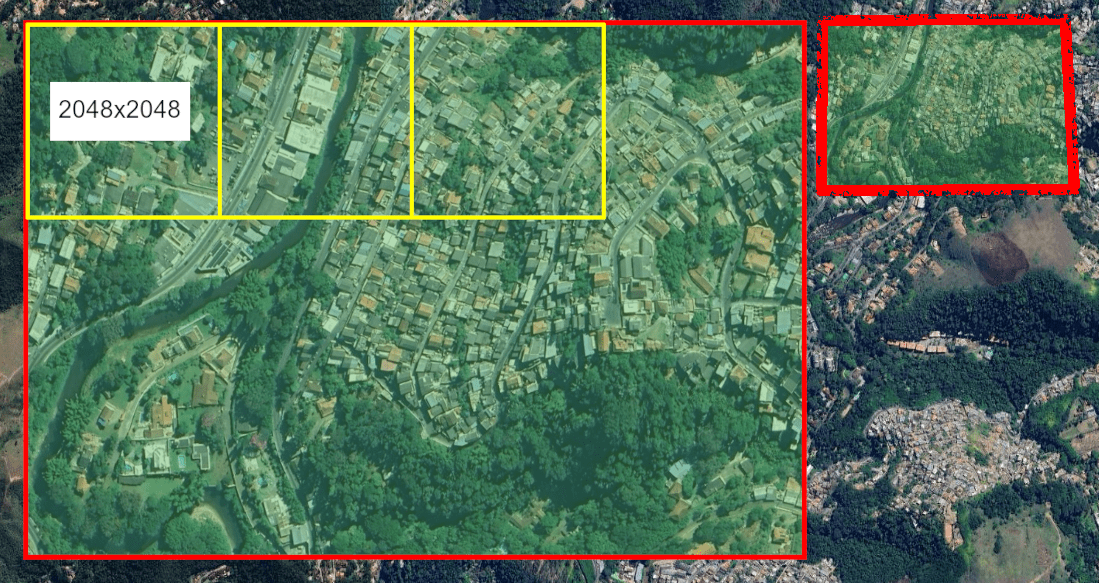
\includegraphics[width = 0.6\columnwidth]{./Figuras/obter_imagens-min}}%% Modo apresentação: tamanho da figura
\mode<article>{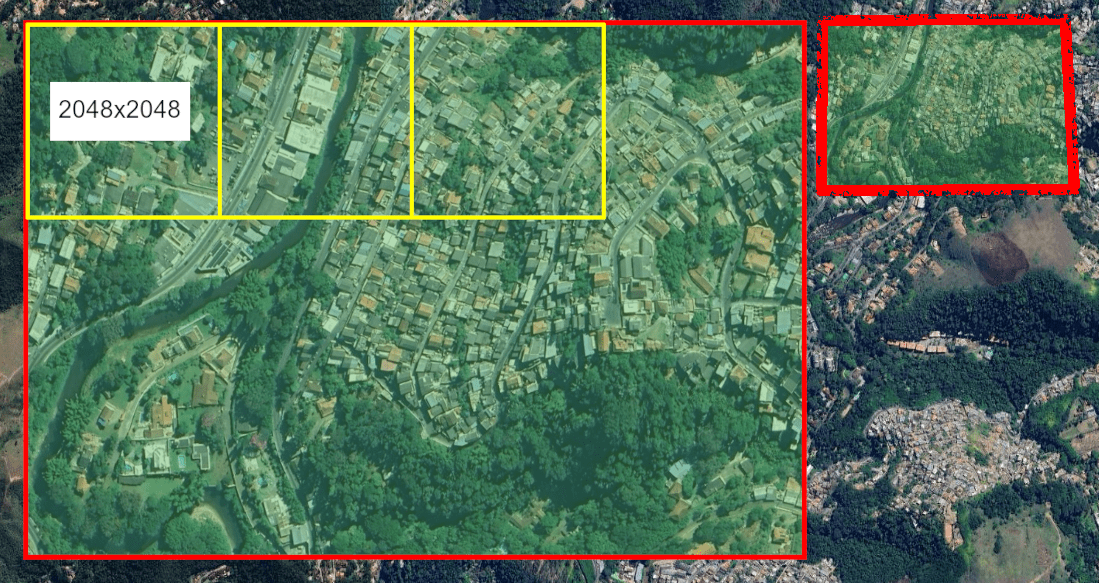
\includegraphics[width = 0.4\columnwidth]{./Figuras/obter_imagens-min}}%% Modo artigo: tamanho da figura
\source{Adaptado de \cite{GE2023}.}
\end{figure}
\end{frame}

\begin{frame}
\begin{columns}[T]
\column{0.5\textwidth}
% A Tabela.~\ref{tab:separacao} apresenta a quantidade de imagens obtidas.
\begin{table}[!htb]
\centering%
\mode<presentation>{\scriptsize}%% Modo apresentação: tamanho de fonte
\mode<article>{\small}%% Modo artigo: tamanho de fonte
\caption{Separação das imagens no conjunto de dados.}%
\label{tab:separacao}
\begin{tabular*}{\columnwidth}{@{\extracolsep{\fill}}lr}
\toprule
Grupo   & Quantidade     \\
\midrule
Treinamento             & 214 ($\approx 67\%$) \\
Teste                   & 42 ($\approx 13\%$) \\
Descontinuadas          & 66 ($\approx 20\%$) \\
Total                   & 322 \\
\bottomrule
\addlinespace
\end{tabular*}
\source{Autoria própria.}
\end{table}
\begin{block}{Mais Detalhes}
    \begin{itemize}
        \item RGB (TIFF).
        \item Resolução padrão de 2048x2048 pixels.
    \end{itemize}
\end{block}
\column{0.5\textwidth}
\begin{figure}[!htb]
\centering%
\caption{Amostras do Conjunto de Dados.}%
\label{fig:obter_imagens}
\mode<presentation>{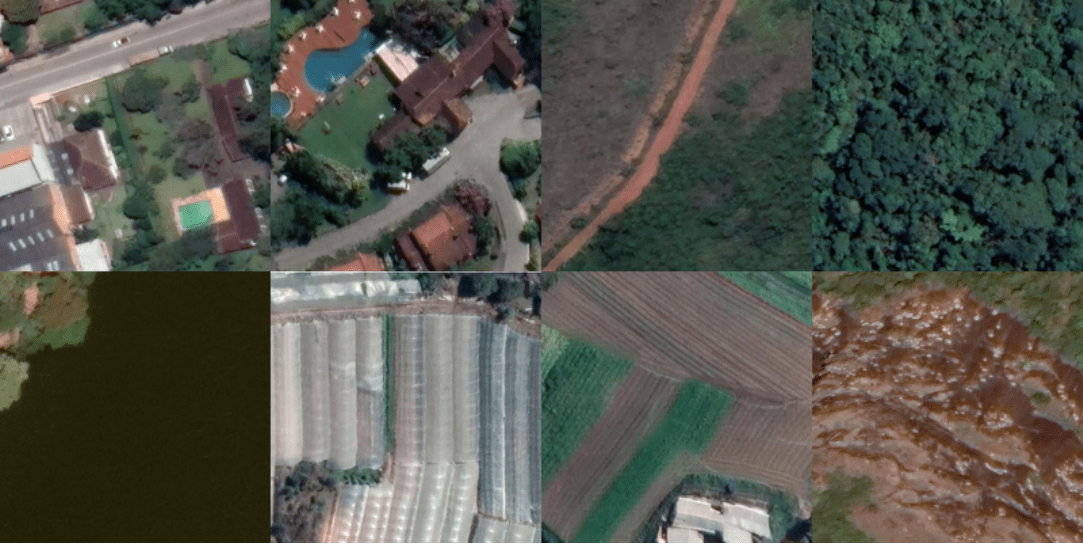
\includegraphics[width = 0.8\columnwidth]{./Figuras/amostras-min}}%% Modo apresentação: tamanho da figura
\mode<article>{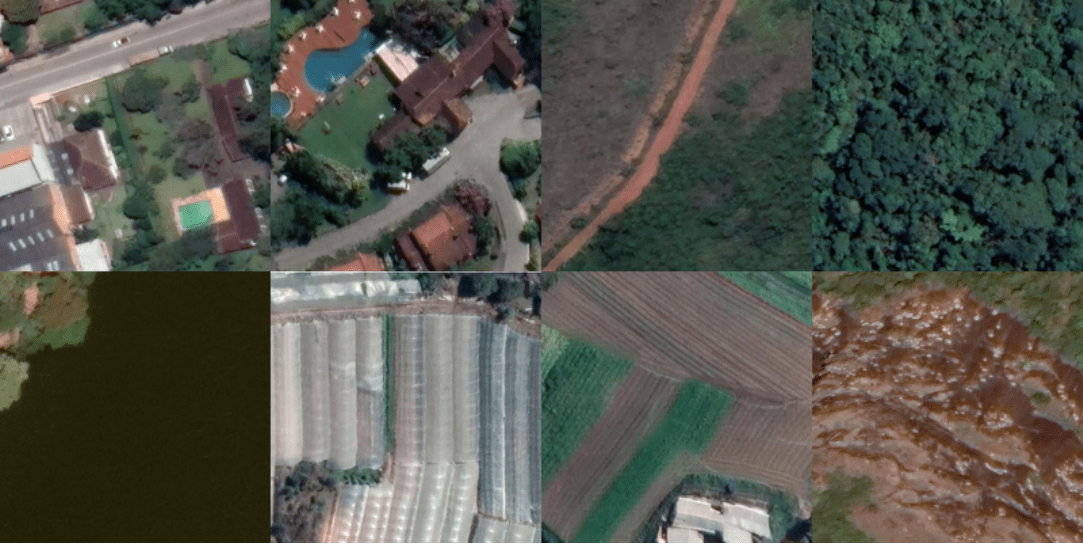
\includegraphics[width = 0.6\columnwidth]{./Figuras/amostras-min}}%% Modo artigo: tamanho da figura
\source{Adaptado de \cite{GE2023}.}
\end{figure}
\end{columns}
\end{frame}

\subsection{Seleção e Rotulagem}\label{ssec:matmet5}

\begin{frame}
\color{black}{\textbf{Seleção}} - \color{gray}{Rotulagem}
\begin{columns}[T]
\column{0.4\textwidth}
\begin{itemize}
    \item Delimitar as regiões de interesse.
    \item Definido em conjunto com equipe do ICMBio.
    \item 8 classes
    \begin{itemize}
        \item Área Desenvolvida
        \item Floresta
        \item Sombra
        \item Área em Regeneração
        \item Solo Exposto
        \item Água
        \item Rocha
        \item Agricultura
        \item \color{red}{Piscina}
    \end{itemize}
\end{itemize}
\column{0.6\textwidth}
\begin{figure}[!htb]
\centering%
\caption{Amostras do Conjunto de Dados por Classe.}%
\label{fig:obter_imagens}
\mode<presentation>{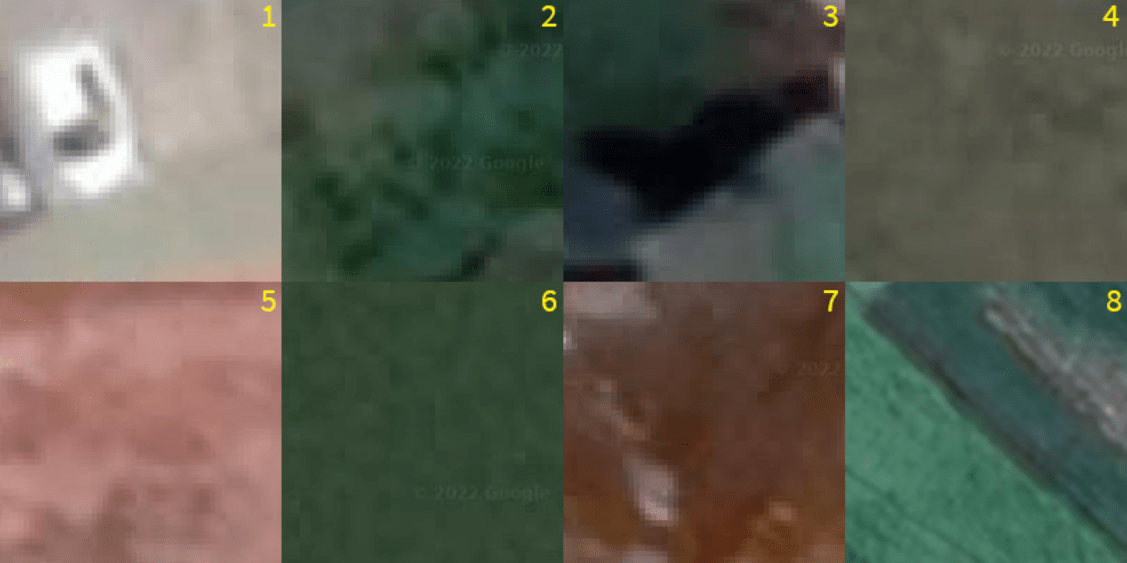
\includegraphics[width = 1.0\columnwidth]{./Figuras/amostras_classe-min}}%% Modo apresentação: tamanho da figura
\mode<article>{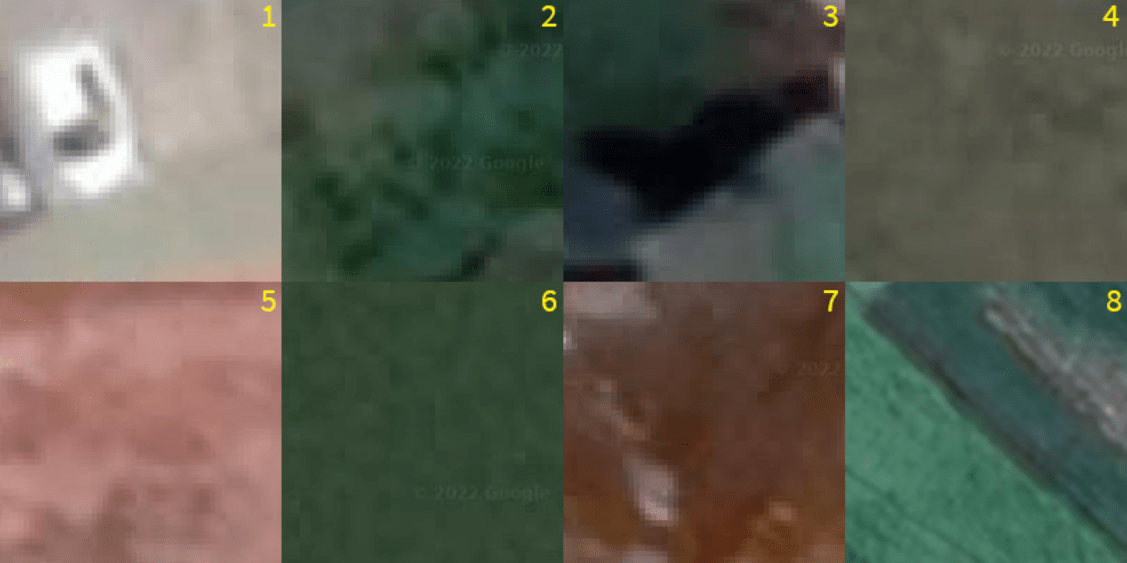
\includegraphics[width = 0.8\columnwidth]{./Figuras/amostras_classe-min}}%% Modo artigo: tamanho da figura
\source{Adaptado de \textcite{GE2023}.}
\end{figure}
\end{columns}
\end{frame}

\begin{frame}
\color{gray}{Seleção} - \color{black}{\textbf{Rotulagem}}

\begin{itemize}
    \item Auxílio de um profissional do ICMBio.
    \item Critério rígido.
    \item Ferramentas
    \begin{itemize}
        \item ArcGis (semi-automático, manual)
        \item CVAT (manual)
    \end{itemize}
\end{itemize}

\begin{figure}[!htb]
\centering%
\caption{Amostra da imagem original e da imagem rotulada.}%
\label{fig:labeled}
\mode<presentation>{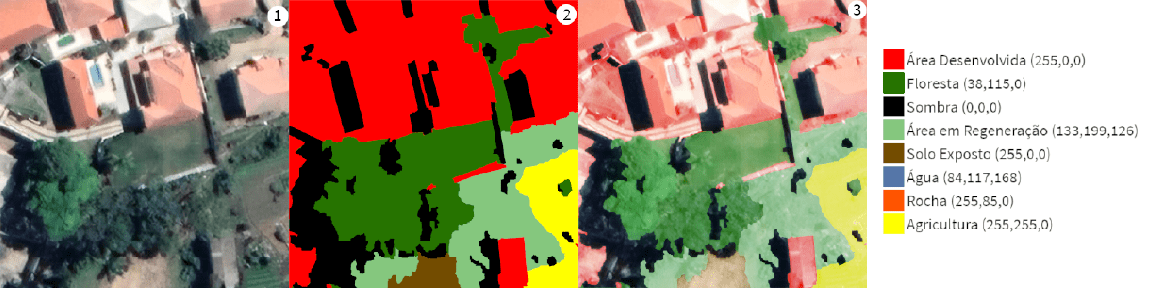
\includegraphics[width = 0.8\columnwidth]{./Figuras/labeled-min}}%% Modo apresentação: tamanho da figura
\mode<article>{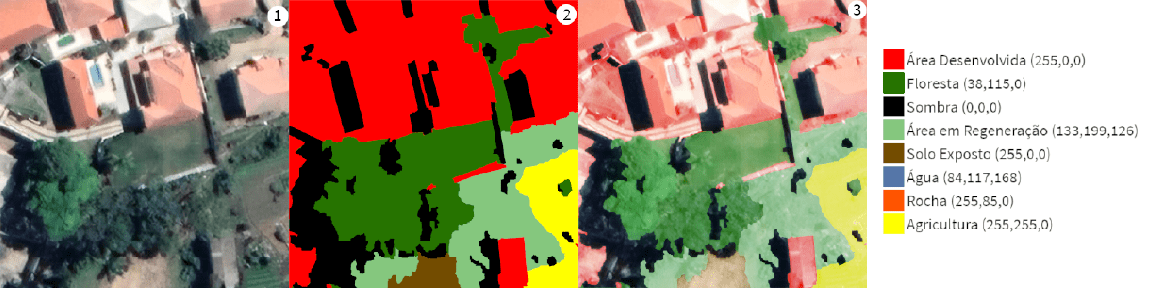
\includegraphics[width = 0.5\columnwidth]{./Figuras/labeled-min}}%% Modo artigo: tamanho da figura
\source{Autoria própria.}
\end{figure}

\end{frame}

\begin{frame}{Metodologia Aplicada no Desbalanceamento de Classes}

\begin{columns}[T]
    
\column{0.6\linewidth}
\begin{itemize}
    \item Método proposto por \cite{Marcatto2022}.
    \item Calcular o peso para cada classe (treinamento).
\end{itemize}

\begin{equation*}\label{eq:met:desbal}
\vcenter{\hbox{\mode<presentation>{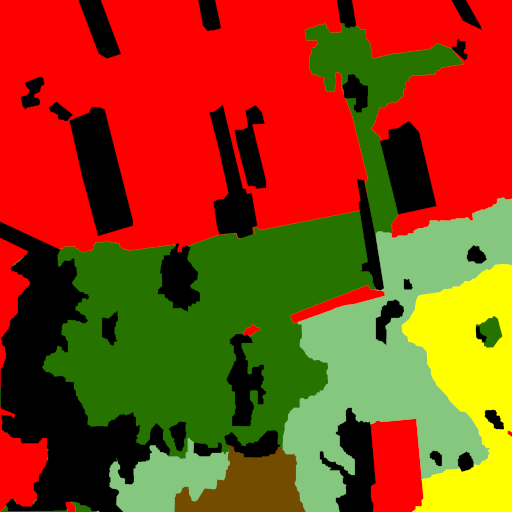
\includegraphics[width=2cm,height=2cm]{./Figuras/239-min}}}}
\vcenter{\hbox{\mode<article>{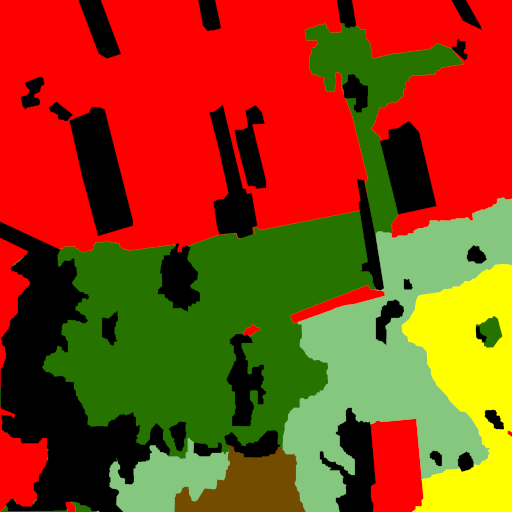
\includegraphics[width=1cm,height=1cm]{./Figuras/239-min}}}}
\qquad\qquad
\begin{aligned}
\varphi(c) = \frac{m}{C*n^{c}}
\end{aligned}
\end{equation*}

\column{0.4\linewidth}
\begin{table}[!htb]
\centering%
\mode<presentation>{\scriptsize}%% Modo apresentação: tamanho de fonte
\mode<article>{\small}%% Modo artigo: tamanho de fonte
\caption{Pesos calculados para o conjunto de treinamento.}%% Legenda
\label{tab:pesos}
\begin{tabular*}{\columnwidth}{@{\extracolsep{\fill}}lr}
\toprule
\textbf{Classe}         & \textbf{Peso}             \\ \midrule
Área Desenvolvida       &       1,1472              \\
Floresta                &       0,3832              \\
Sombra                  &       2,0468              \\
Área em Regeneração     &       0,4436              \\
Agricultura             &       1,4859              \\
Rocha                   &       2,4287              \\
Solo Exposto            &       \colorbox{yellow}{5,2043}              \\ 
Água                    &       2,0031              \\
\bottomrule
\addlinespace
\end{tabular*}
\source{Autoria própria.}
\end{table}

\end{columns}

\noindent
em que $m$ é o número de pixels de todas as imagens de treinamento, $C$ é o número de classes, e $n^c$ é o número de pixels que pertencem à classe $c$.

\end{frame}

\subsection{Implementação e Adaptações na Rede SegNet e U-NET}\label{ssec:matmet6}

\begin{frame}

\begin{itemize}
    \item \textbf{MPSegnet} proposta por \textbf{\textcite{Andre2021}}
    \item Uma nova estratégia de multi-pooling, substituindo o max-pooling por \textit{Discrete Wavelet Transform} (DWT) e unpooling por \textit{Inverse Discrete Wavelet Transform} (IWT).
    \item Conjunto de dados utilizado nos experimentos
    \begin{itemize}
        \item 2D Semantic Labeling Contest - Potsdam 
        \item IRRG: 3 canais (IR-R-G)
    \end{itemize}
\end{itemize}

\begin{figure}[!htb]
\centering%
\caption{Arquitetura da MPSegnet.}%
\label{fig:graficoxy1}
\mode<presentation>{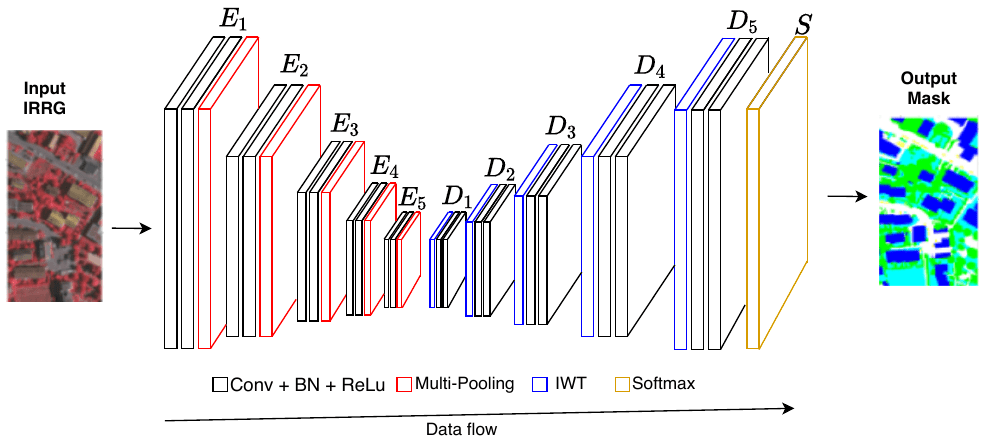
\includegraphics[width = 0.5\columnwidth]{./Figuras/mpsegnet-min}}%% Modo apresentação: tamanho da figura
\mode<article>{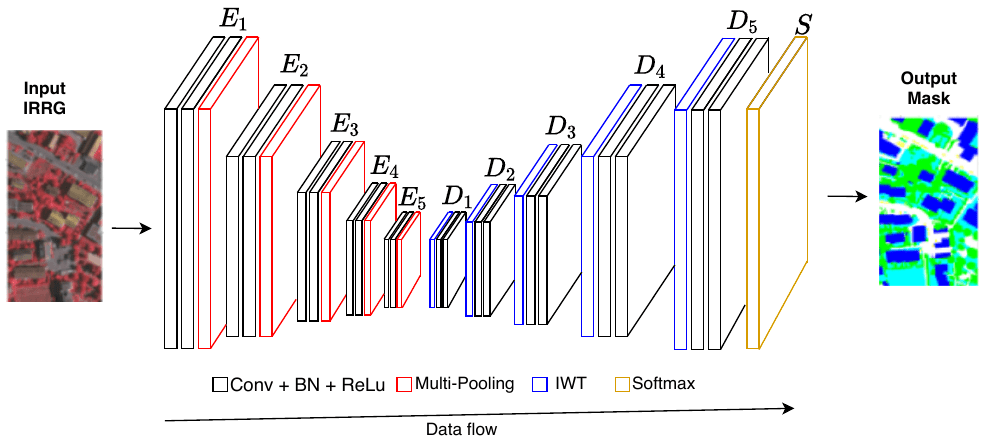
\includegraphics[width = 0.5\columnwidth]{./Figuras/mpsegnet-min}}%% Modo artigo: tamanho da figura
\source{\cite{Andre2021}}
\end{figure}

\end{frame}

\begin{frame}

\begin{itemize}
    \item \textbf{U-NET} sugerida no artigo de \textbf{\textcite{Khanh2021}}.
    \item Combinação de \textbf{EfficientNet-B0} \cite{EfficientNet} (ENCODER) para extração de características com \textbf{U-NET} \cite{Unet2015} (DECODER) para reconstrução do mapa de características.
    \item Conjunto de dados utilizado nos experimentos
    \begin{itemize}
        \item Imagens Aéreas (Google Earth)
        \item RGB: 3 canais (\textit{Red-Green-Blue})
    \end{itemize}
\end{itemize}

\begin{columns}[T]
\column{0.5\linewidth}

\begin{table}[!htb]
\centering%
\mode<presentation>{\scriptsize}%% Modo apresentação: tamanho de fonte
\mode<article>{\small}%% Modo artigo: tamanho de fonte
\caption{Comparativo entre \textit{encoder} e funções de custo.}%
\label{tab:met:unet}
\begin{tabular*}{\columnwidth}{@{\extracolsep{\fill}}lrrrr}
\toprule
\textit{ENCODER}    & Parâmetros    & Categorical Cross & Dice & Average    \\ 
                    &               & Entropy Loss      & Loss & Loss       \\
\midrule
VGG11       & 32M         & 1.194               & 0.770             & 1.066             \\
ResNet18    & 18M         & 1.191               & 0.770             & 1.065             \\
EffNet-B0   & \textbf{4M} & \textbf{1.110}      & \textbf{0.731}    & \textbf{0.997}    \\
EffNet-B1   & 6.5M        & 1.374               & 0.806             & 1.204             \\
EffNet-B2   & 8M          & 1.134               & 0.747             & 1.018             \\
\bottomrule
\addlinespace
\end{tabular*}
\source{Adaptado de \textcite{Khanh2021}.}
\end{table}

\end{columns}
\end{frame}

\subsection{Treinamento e Teste}\label{ssec:matmet7}

\begin{frame}
\begin{itemize}
    \item Conjunto de dados dividido em treinamento e teste (Ver Tabela \ref{tab:separacao}).
    % \item Pré-processamento: Protocolo de \textbf{janelas deslizantes} adotado também no trabalho de \textcite{Andre2021}.
    \item Pré-processamento: \textbf{10.000} amostras de \textbf{256x256} (recortes aleatórios).
    \item Inicialização dos pesos: Pesos pré-treinados na ImageNet \cite{Imagenet2009}.
\end{itemize}

\begin{columns}[T]
\column{0.4\linewidth}

\begin{block}{Treinamento}
    \begin{itemize}
        \item Conjunto de dados embaralhado.
        \item Aumento de dados
        \begin{itemize}
            \item \textbf{Espelhamento horizontal e vertical}
        \end{itemize}
    \end{itemize}
\end{block}

\column{0.5\linewidth}
\begin{block}{Teste}
    \begin{itemize}
        \item Conjunto de dados \textbf{não} é embaralhado.
        \item Sem aumento de dados.
        \item Protocolo de janelas deslizantes sobrepostas com passo de 32 pixels para evitar inconsistências na segmentação, especialmente nas bordas \cite{Farhangfar2019}.
        \item Maior esforço computacional.
    \end{itemize}
\end{block}

\end{columns}
\end{frame}

\begin{frame}
% \frametitle<presentation>{Frame Title Should Be in Uppercase.}
\framesubtitle{Treinamento e Teste - Mais detalhes de implementação.}

\begin{itemize}
    \item \textbf{Número de classes}: 8
    \item \textbf{Épocas de treinamento}: 100
    \item \textbf{Tamanho do \textit{batch}}: 8
    \item \textbf{Taxa de aprendizagem}: 1e-2
    \begin{itemize}
        \item \textbf{Escalonamento}: redução de 10 vezes nas 25°, 35° e 45° épocas
        \item \textbf{Decaimento}: limitado a 1e-5
    \end{itemize}
    \item \textbf{Otimizador}: SGD (\textit{Stochastic Gradient Descent})
    \begin{itemize}
        \item \textit{Momentum}: 0,9
        \item \textit{Weight Decay}: 1e-5
    \end{itemize}
\end{itemize}

\begin{block}{Observações}
    Os detalhes de implementação acima foram utilizados em ambos os modelos e consideraram as escolhas de \textcite{Andre2021}.
\end{block}
       
\end{frame}

\begin{frame}
\framesubtitle{Função de Custo - Entropia Cruzada}

Mede a diferença entre a distribuição de probabilidade prevista (\(p_i\)) e o \textit{ground truth} dos rótulos para a classe (\(y_i\)), comumente expressa pela Equação \ref{eq:celoss} \cite{Celoss2019}.

% \begin{block}{Supondo que}
%     \(D = \{(x_1, y_1), ..., (x_i, y_i), ..., (x_M, y_M)\}\), onde \(y_i\) é um vetor representando o rótulo da \(i\)-ésima amostra \(x_i\), \(p_{ij}\) representa a probabilidade de que a amostra \(x_i\) seja atribuída à \(j\)-ésima classe, onde \(j\) varia de 1 a \(M\), sendo \(M\) o número total de classes.
% \end{block}

\begin{equation}\label{eq:celoss}
L_{CE} = -\frac{1}{M}\sum_{i=1}^{M}\left ( y_i^{T} log\left ( p_i \right ) \right )
\end{equation}

\noindent
onde \(M\) é o número total de classes, \(L_{CE}\) é a função de entropia cruzada, \(y_i^{T}\) é o vetor (\textit{ground truth}) transposto de \(y_i\), \(p\) é o vetor de probabilidades atribuídas a cada classe.

\end{frame}

\begin{frame}
\framesubtitle{Função de Custo - \textit{Focal Loss}}

É uma modificação da função de entropia cruzada que visa resolver o problema de desbalanceamento de classes, dando maior peso às classes minoritárias. A função é definida pela Equação \ref{eq:focal} \cite{FocalLoss2020}.

\begin{equation}\label{eq:focal}
FL(p_t) = -\sum_{i=1}^{C} (1 - p_{ti})^\gamma \cdot \log(p_{ti})
\end{equation}

\noindent
onde:
\begin{itemize}
    \item \(C\) é o número de classes.
    \item \(p_ti\) é a probabilidade prevista da classe verdadeira.
    \item \(\gamma\) é um parâmetro de foco ajustável.
    \item O termo \((1 - p_ti)^\gamma\) reduz o peso da perda para exemplos bem classificados, focando mais nos exemplos difíceis e mal classificados.
    \item Quando \(p_t\) está próximo de 1 (indicando uma previsão confiante e correta), a perda é reduzida.
\end{itemize}

Isso ajuda a reduzir o impacto de pixels fáceis de classificar e permite que o modelo se concentre mais em regiões desafiadoras.

\end{frame}

\section{Resultados e Discussão}\label{sec:resuldisc}

\subsection{Cenários}\label{ssec:resuldisc1}

\begin{frame}

\begin{itemize}
    \item \textbf{Cenário 1}: SegNet Modificada, usando a função de custo \textbf{Entropia Cruzada}.
    \begin{itemize}
        \item Experimento 1: \textbf{pesos iguais (1)}.
        \item Experimento 2: \textbf{pesos ponderados}. 
        \item Utilização de 9 classes (8 classes + \colorbox{yellow}{piscina}).
    \end{itemize}
\end{itemize}
\begin{itemize}
    \item \textcolor{lightgray}{\textbf{Cenário 2}: SegNet Modificada, usando a função de custo \textbf{Entropia Cruzada}.}
    \begin{itemize}
        \item \textcolor{lightgray}{Experimento 1: \textbf{com aumento de dados}.}
        \item \textcolor{lightgray}{Experimento 2: \textbf{sem aumento de dados}.}
        \item \textcolor{lightgray}{Ambos usam pesos ponderados na função de custo.}
    \end{itemize}
\end{itemize}
\begin{itemize}
    \item \textcolor{lightgray}{\textbf{Cenário 3}: U-NET, usando a função de custo \textbf{Entropia Cruzada} com pesos ponderados.}
    \begin{itemize}
        \item \textcolor{lightgray}{Experimento 1: \textbf{com aumento de dados}.}
        \item \textcolor{lightgray}{Experimento 2: \textbf{sem aumento de dados}.}
    \end{itemize}
\end{itemize}
\begin{itemize}
    \item \textcolor{lightgray}{\textbf{Cenário 4}: SegNet Modificada e U-NET, usando a função de custo \textbf{Focal Loss}.}
    \begin{itemize}
        \item \textcolor{lightgray}{Experimento 1: SegNet Modificada \textbf{com aumento de dados}.}
        \item \textcolor{lightgray}{Experimento 2: U-NET \textbf{com aumento de dados}.}
    \end{itemize}
\end{itemize}

% \begin{block}{Observações}
%     Aumento de dados: \textbf{Espelhamento horizontal e vertical}.
% \end{block}
\end{frame}

\begin{frame}
\framesubtitle{Cenário 1 - Distribuição de pesos na função de custo}

\begin{table}[!ht]
    \centering
    \mode<presentation>{\scriptsize}%% Modo apresentação: tamanho de fonte
    \mode<article>{\small}%% Modo artigo: tamanho de fonte
    \caption{Pesos ponderados para a função de custo no cenário 1.}%% Legenda
    \label{tab:res:cen1:pesos}%% Rótulo
    \begin{tabular}{ll}
    \toprule
        \textbf{Classe}                     & \textbf{Peso} \\ \midrule
        \textbf{Área Desenvolvida}          & 0,9786 \\ 
        \textbf{Floresta}                   & 0,3264 \\ 
        \textbf{Piscina}                    & \colorbox{yellow}{51,3827} \\ 
        \textbf{Sombra}                     & 1,7031 \\ 
        \textbf{Área em Regeneração}        & 0,3702 \\ 
        \textbf{Agricultura}                & 1,2344 \\ 
        \textbf{Rocha}                      & 2,0176 \\ 
        \textbf{Solo Exposto}               & 4,8396 \\ 
        \textbf{Água}                       & 10,5859 \\
        \bottomrule
        \addlinespace
    \end{tabular}
    \source{Autoria própria.}%% Fonte
\end{table}

\begin{block}{Observações}
    \begin{itemize}
        \item \textbf{Piscina}: maior peso.
        \item Os demais cenários consideram os pesos calculados e apresentados na \textbf{Tabela \ref{tab:pesos}}.
    \end{itemize}
\end{block}
\end{frame}

\begin{frame}
\framesubtitle{Cenário 1 - Análise dos Resultados}
\begin{columns}[T]

\column{0.5\linewidth}
\begin{table}[!ht]
    \centering
    \mode<presentation>{\scriptsize}%% Modo apresentação: tamanho de fonte
    \mode<article>{\small}%% Modo artigo: tamanho de fonte
    \caption{Resultados da SegNet no cenário 1 com pesos iguais.}%% Legenda
    \label{tab:res:cen11}%% Rótulo
    % \begin{tabular*}{\columnwidth}{@{\extracolsep{\fill}}llllll}
    \begin{tabular}{lllll}
    \toprule
        \textbf{Classe} & \textbf{Prec} & \textbf{Sens} & \textbf{F1-Score} & \textbf{IoU} \\
        \midrule
        \textbf{Desenvolvida} & 0.79 & 0.80 & 0.80 & 0.66  \\ 
        \textbf{Floresta} & 0.89 & 0.87 & 0.88 & 0.78  \\ 
        \textbf{Piscina} & \colorbox{yellow}{0.18}\footnote<.->{Proporção de VP mantida em ambos os experimentos.} & 0.89 & 0.30 & 0.17  \\ 
        \textbf{Sombra} & 0.86 & 0.80 & 0.83 & 0.70  \\ 
        \textbf{Regeneração} & 0.73 & 0.89 & 0.80 & 0.66  \\ 
        \textbf{Agricultura} & 0.82 & 0.83 & 0.82 & 0.70  \\ 
        \textbf{Rocha} & 0.86 & 0.45 & 0.59 & 0.42  \\ 
        \textbf{Solo Exposto} & 0.56 & 0.20 & 0.29 & 0.17  \\ 
        \textbf{Água} & 0.45 & \colorbox{red!25}{0.06} & \colorbox{red!25}{0.11} & 0.05 \\ 
        \textbf{} & ~ & ~ & ~ & ~ \\ 
        \textbf{Acurácia} & \colorbox{green!25}{0.81}\footnote<.->{Ponderação nos pesos pode ter afetado a acurácia.} & ~ & \textbf{IoU} & 0.48 \\
        \bottomrule
        \addlinespace
    \end{tabular}
    \source{Autoria própria.}%% Fonte
\end{table}

\column{0.5\linewidth}

\begin{table}[!ht]
    \centering
    \mode<presentation>{\scriptsize}%% Modo apresentação: tamanho de fonte
    \mode<article>{\small}%% Modo artigo: tamanho de fonte
    \caption{Resultados da SegNet no cenário 2 com pesos ponderados.}%% Legenda
    \label{tab:res:cen12}%% Rótulo
    \begin{tabular}{lllll}
    \toprule
        \textbf{Classe} & \textbf{Prec} & \textbf{Sens} & \textbf{F1-Score} & \textbf{IoU} \\
        \midrule
        \textbf{Desenvolvida}               & 0.71 & 0.76 & 0.73 & 0.57  \\ 
        \textbf{Floresta}                   & 0.89 & 0.67 & 0.76 & 0.61  \\ 
        \textbf{Piscina}                    & \colorbox{yellow}{0.18} & 0.99 & 0.30 & 0.18  \\ 
        \textbf{Sombra}                     & 0.60 & 0.86 & 0.71 & 0.55  \\ 
        \textbf{Regeneração}                & 0.80 & 0.44 & 0.56 & 0.39  \\ 
        \textbf{Agricultura}                & 0.66 & 0.76 & 0.70 & 0.54  \\ 
        \textbf{Rocha}                      & 0.37 & 0.69 & 0.48 & 0.31  \\ 
        \textbf{Solo Exposto}               & 0.09 & 0.40 & 0.14 & 0.08  \\ 
        \textbf{Água}                       & 0.46 & \colorbox{green!25}{0.73}\footnote<.->{Redução significativa nos falsos negativos} & \colorbox{green!25}{0.56}\footnote<.->{Melhor equilíbrio entre precisão e sensibilidade} & \colorbox{green!25}{0.39}\footnote<.->{Melhoria na sobreposição entre \textit{Ground Truth} e previsão na segmentação.} \\ 
        \textbf{} & ~ & ~ & ~ &  ~ \\ 
        \textbf{Acurácia} & \colorbox{red!25}{0.65} & ~ & \textbf{IoU} & 0.40 \\
        \bottomrule
        \addlinespace
    \end{tabular}
    \source{Autoria própria.}%% Fonte
\end{table}

\end{columns}
\end{frame}

\begin{frame}
\framesubtitle{Cenário 1 - Matriz de Confusão}

\begin{columns}[T]

\column{0.5\linewidth}
\begin{figure}[!htb]
\centering%
\caption{Matriz de confusão do cenário 1 com pesos iguais.}%
\label{fig:matriz:cen11}
\mode<presentation>{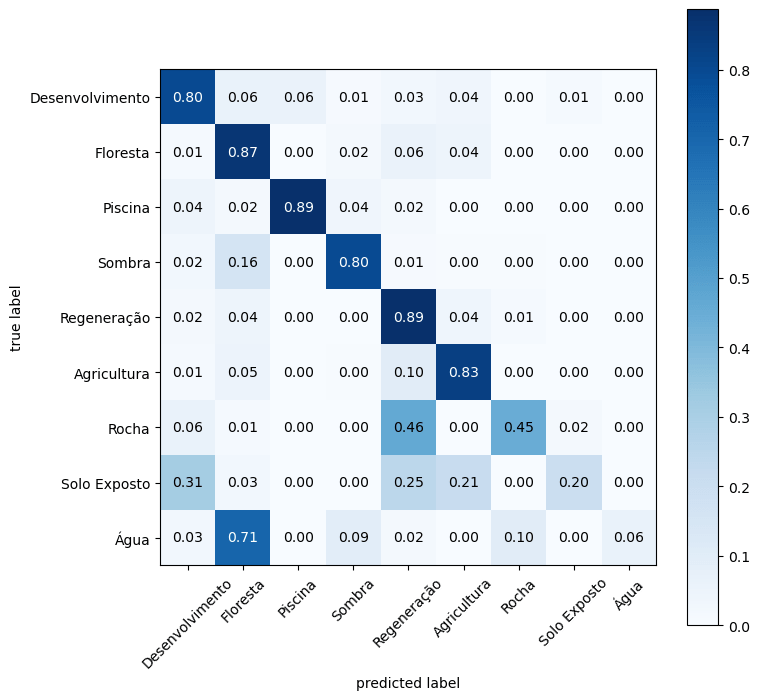
\includegraphics[width = 0.8\columnwidth]{./Figuras/cm/cm_cenario_11-min.png}}%% Modo apresentação: tamanho da figura
\mode<article>{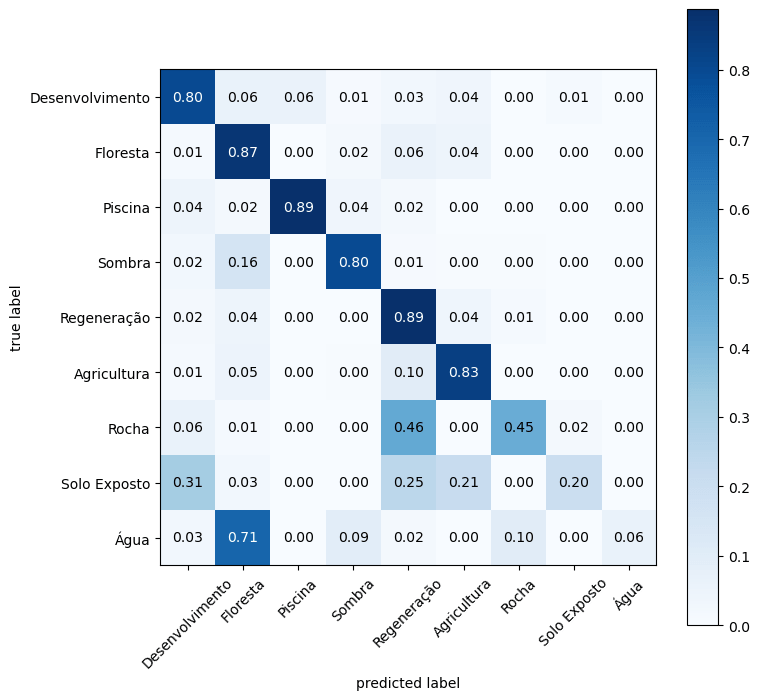
\includegraphics[width = 0.5\columnwidth]{./Figuras/cm/cm_cenario_11-min.png}}%% Modo artigo: tamanho da figura
\source{Autoria própria.}
\end{figure}

\column{0.5\linewidth}

\begin{figure}[!htb]
\centering%
\caption{Matriz de confusão do cenário 2 com pesos ponderados.}%
\label{fig:matriz:cen12}
\mode<presentation>{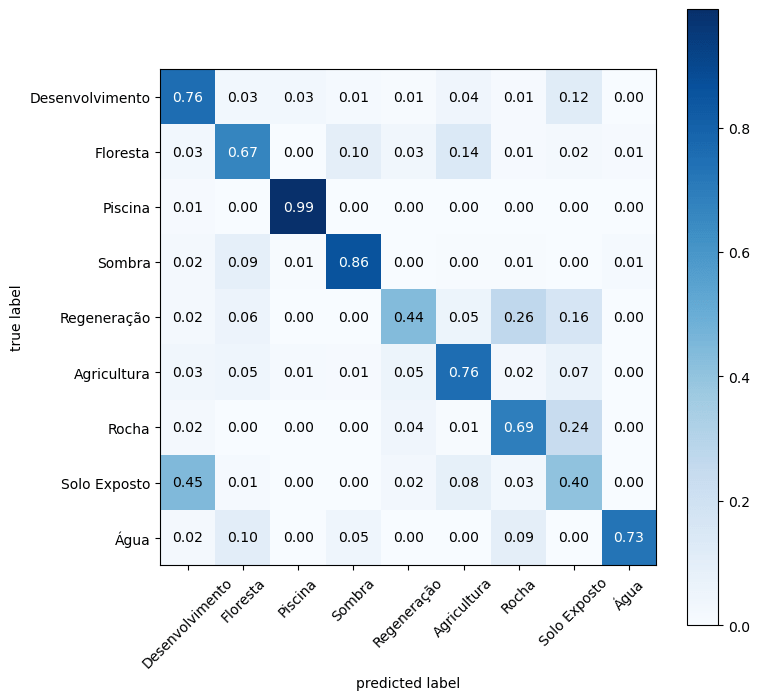
\includegraphics[width = 0.8\columnwidth]{./Figuras/cm/cm_cenario_12-min.png}}%% Modo apresentação: tamanho da figura
\mode<article>{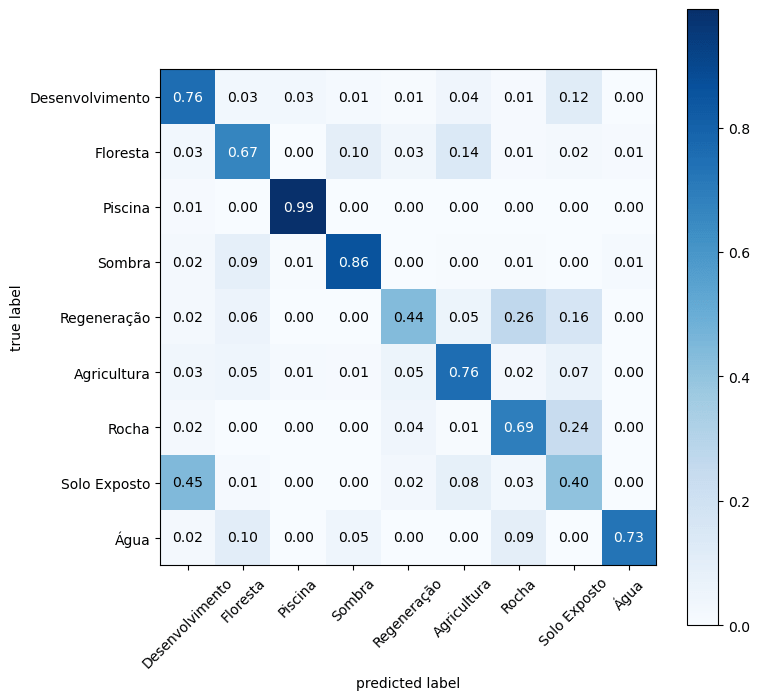
\includegraphics[width = 0.5\columnwidth]{./Figuras/cm/cm_cenario_12-min.png}}%% Modo artigo: tamanho da figura
\source{Autoria própria.}
\end{figure}

\end{columns}
\end{frame}

\begin{frame}

    \begin{itemize}
        \item \textcolor{lightgray}{\textbf{Cenário 1}: SegNet Modificada, usando a função de custo \textbf{Entropia Cruzada}.}
        \begin{itemize}
            \item \textcolor{lightgray}{Experimento 1: \textbf{pesos iguais (1)}.}
            \item \textcolor{lightgray}{Experimento 2: \textbf{pesos ponderados}.}
            \item \textcolor{lightgray}{Utilização de 9 classes (8 classes + \colorbox{yellow}{piscina}).}
        \end{itemize}
    \end{itemize}
    \begin{itemize}
        \item \textbf{Cenário 2}: SegNet Modificada, usando a função de custo \textbf{Entropia Cruzada}.
        \begin{itemize}
            \item Experimento 1: \textbf{com aumento de dados}.
            \item Experimento 2: \textbf{sem aumento de dados}.
            \item Ambos usam pesos ponderados na função de custo.
        \end{itemize}
    \end{itemize}
    \begin{itemize}
        \item \textcolor{lightgray}{\textbf{Cenário 3}: U-NET, usando a função de custo \textbf{Entropia Cruzada} com pesos ponderados.}
        \begin{itemize}
            \item \textcolor{lightgray}{Experimento 1: \textbf{com aumento de dados}.}
            \item \textcolor{lightgray}{Experimento 2: \textbf{sem aumento de dados}.}
        \end{itemize}
    \end{itemize}
    \begin{itemize}
        \item \textcolor{lightgray}{\textbf{Cenário 4}: SegNet Modificada e U-NET, usando a função de custo \textbf{Focal Loss}.}
        \begin{itemize}
            \item \textcolor{lightgray}{Experimento 1: SegNet Modificada \textbf{com aumento de dados}.}
            \item \textcolor{lightgray}{Experimento 2: U-NET \textbf{com aumento de dados}.}
        \end{itemize}
    \end{itemize}
    
    % \begin{block}{Observações}
    %     Aumento de dados: \textbf{Espelhamento horizontal e vertical}.
    % \end{block}
    \colorbox{yellow}{Aumento de dados: \textbf{Espelhamento horizontal e vertical}.}
\end{frame}

\begin{frame}
\framesubtitle{Cenário 2 - Análise dos Resultados}

\begin{columns}[T]

\column{0.5\linewidth}
\begin{table}[!ht]
    \centering
    \mode<presentation>{\scriptsize}%% Modo apresentação: tamanho de fonte
    \mode<article>{\small}%% Modo artigo: tamanho de fonte
    \caption{Resultados da SegNet no cenário 2 com aumento de dados.}%% Legenda
    \label{tab:res:cen12}%% Rótulo
    \begin{tabular}{lllll}
    \toprule
        \textbf{Classe} & \textbf{Prec} & \textbf{Sens} & \textbf{F1-Score} & \textbf{IoU} \\
        \midrule
        \textbf{Desenvolvida} & 0.83 & 0.77 & 0.80 & 0.66  \\ 
        \textbf{Floresta} & 0.94 & 0.77 & 0.85 & 0.74  \\ 
        \textbf{Sombra} & 0.69 & 0.93 & 0.79 & 0.66  \\ 
        \textbf{Regeneração} & 0.83 & 0.66 & 0.73 & 0.58  \\ 
        \textbf{Agricultura} & 0.83 & 0.77 & 0.80 & 0.66  \\ 
        \textbf{Rocha} & 0.50 & 0.77 & 0.61 & 0.43 \\ 
        \textbf{Solo Exposto} & 0.17 & 0.79 & 0.28 & 0.16 \\ 
        \textbf{Água} & 0.72 & 0.89 & 0.79 & 0.66 \\ 
        \textbf{} & ~ & ~ & ~ & ~ \\ 
        \textbf{Acurácia} & 0.76 & ~ & \textbf{IoU} & 0.57 \\
        \bottomrule
        \addlinespace
    \end{tabular}
    \source{Autoria própria.}%% Fonte
\end{table}

\column{0.5\linewidth}

\begin{table}[!ht]
    \centering
    \mode<presentation>{\scriptsize}%% Modo apresentação: tamanho de fonte
    \mode<article>{\small}%% Modo artigo: tamanho de fonte
    \caption{Resultados da SegNet no cenário 2 sem aumento de dados.}%% Legenda
    \label{tab:res:cen22}%% Rótulo
    \begin{tabular}{lllll}
    \toprule
        \textbf{Classe} & \textbf{Prec} & \textbf{Sens} & \textbf{F1-Score} & \textbf{IoU} \\
        \midrule
        \textbf{Desenvolvida}    & \textbf{0.84} & \textbf{0.84} & \textbf{0.84} & \textbf{0.72}  \\ 
        \textbf{Floresta}        & \textbf{0.95} & 0.76 & \textbf{0.85} & 0.73  \\ 
        \textbf{Sombra}          & \textbf{0.70} & 0.92 & \textbf{0.80} & \textbf{0.67}  \\ 
        \textbf{Regeneração}     & \textbf{0.88} & 0.65 & \textbf{0.75} & \textbf{0.60}  \\ 
        \textbf{Agricultura}     & 0.72 & \textbf{0.93} & \textbf{0.81} & \textbf{0.69}  \\ 
        \textbf{Rocha}           & \textbf{0.55} & \textbf{0.83} & \textbf{0.66} & \textbf{0.50}  \\ 
        \textbf{Solo Exposto}    & \textbf{0.27} & 0.73 & \textbf{0.40} & \textbf{0.25}  \\ 
        \textbf{Água}            & \textbf{0.89} & \colorbox{green!25}{0.95} & \colorbox{green!25}{0.92} & \colorbox{green!25}{0.85} \\ 
        \textbf{} & ~ & ~ & ~ & ~ \\ 
        \textbf{Acurácia} & \colorbox{green!25}{0.79} & ~ & \textbf{IoU} & \colorbox{green!25}{0.62} \\
        \bottomrule
        \addlinespace
    \end{tabular}
    \source{Autoria própria.}%% Fonte
\end{table}

\end{columns}
\end{frame}

\begin{frame}
\framesubtitle{Cenário 2 - Matriz de Confusão}

\begin{columns}[T]

\column{0.5\linewidth}
\begin{figure}[!htb]
\centering%
\caption{Matriz de confusão do cenário 2 com aumento de dados.}%
\label{fig:matriz:cen21}
\mode<presentation>{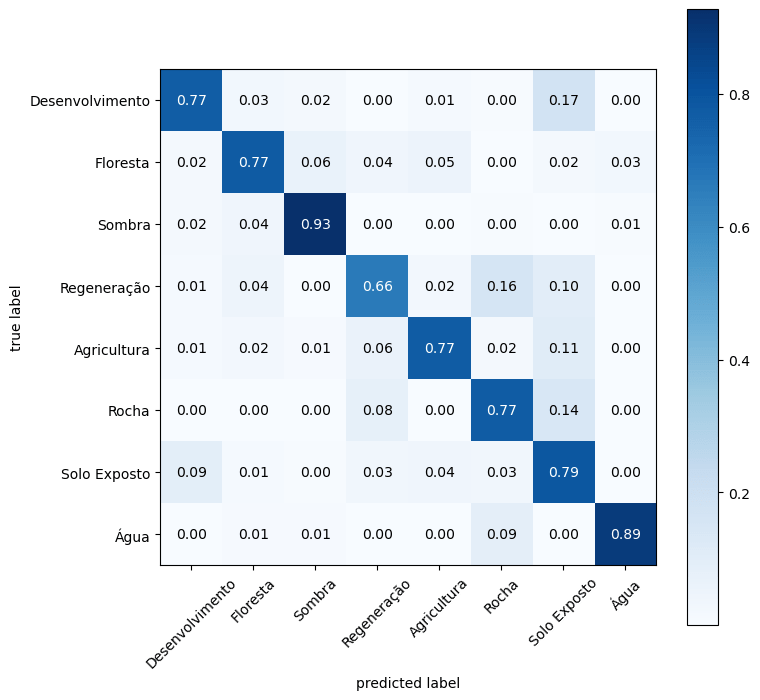
\includegraphics[width = 0.8\columnwidth]{./Figuras/cm/cm_cenario_21-min.png}}%% Modo apresentação: tamanho da figura
\mode<article>{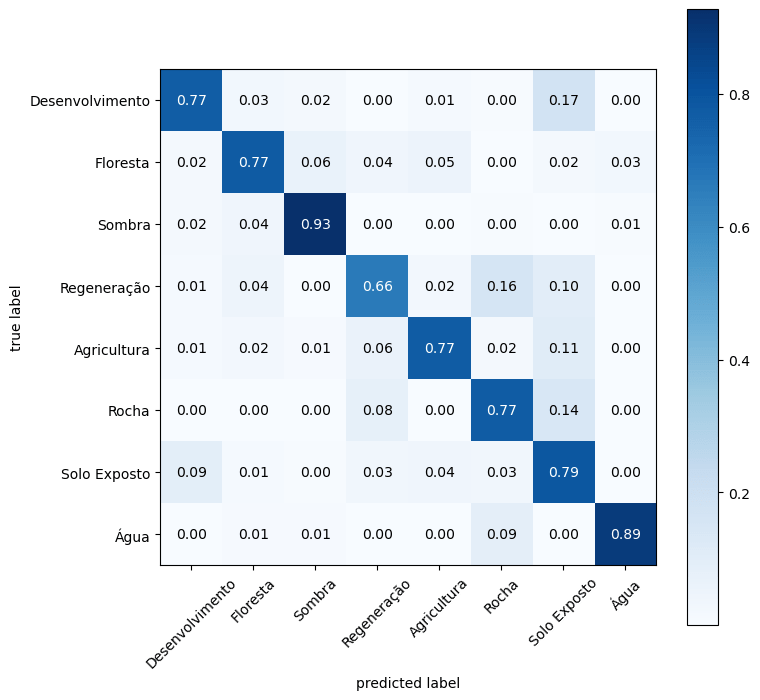
\includegraphics[width = 0.5\columnwidth]{./Figuras/cm/cm_cenario_21-min.png}}%% Modo artigo: tamanho da figura
\source{Autoria própria.}
\end{figure}

\column{0.5\linewidth}

\begin{figure}[!htb]
\centering%
\caption{Matriz de confusão do cenário 2 sem aumento de dados.}%
\label{fig:matriz:cen22}
\mode<presentation>{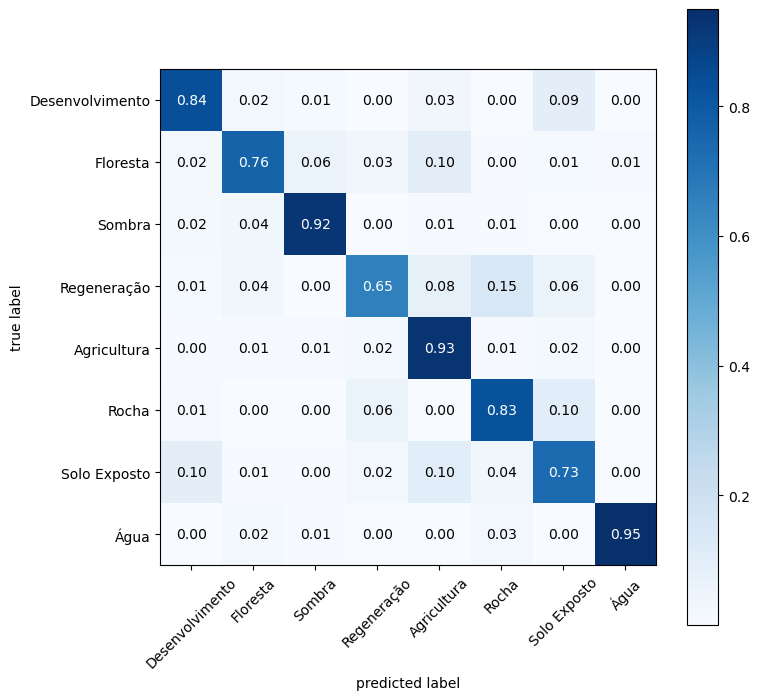
\includegraphics[width = 0.8\columnwidth]{./Figuras/cm/cm_cenario_22-min.png}}%% Modo apresentação: tamanho da figura
\mode<article>{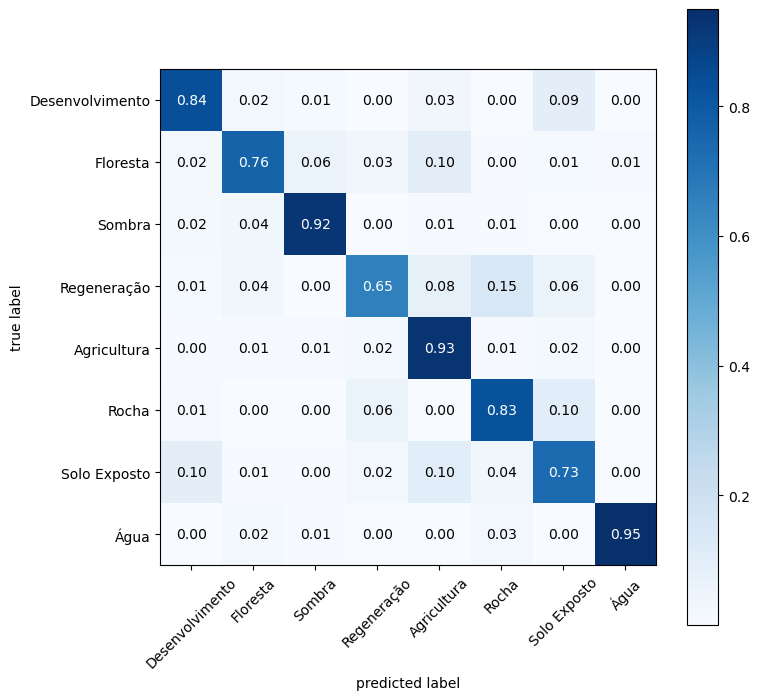
\includegraphics[width = 0.5\columnwidth]{./Figuras/cm/cm_cenario_22-min.png}}%% Modo artigo: tamanho da figura
\source{Autoria própria.}
\end{figure}

\end{columns}
\end{frame}

\begin{frame}

    \begin{itemize}
        \item \textcolor{lightgray}{\textbf{Cenário 1}: SegNet Modificada, usando a função de custo \textbf{Entropia Cruzada}.}
        \begin{itemize}
            \item \textcolor{lightgray}{Experimento 1: \textbf{pesos iguais (1)}.}
            \item \textcolor{lightgray}{Experimento 2: \textbf{pesos ponderados}.}
            \item \textcolor{lightgray}{Utilização de 9 classes (8 classes + \colorbox{yellow}{piscina}).}
        \end{itemize}
    \end{itemize}
    \begin{itemize}
        \item \textcolor{lightgray}{\textbf{Cenário 2}: SegNet Modificada, usando a função de custo \textbf{Entropia Cruzada}.}
        \begin{itemize}
            \item \textcolor{lightgray}{Experimento 1: \textbf{com aumento de dados}.}
            \item \textcolor{lightgray}{Experimento 2: \textbf{sem aumento de dados}.}
            \item \textcolor{lightgray}{Ambos usam pesos ponderados na função de custo.}
        \end{itemize}
    \end{itemize}
    \begin{itemize}
        \item \textbf{Cenário 3}: U-NET, usando a função de custo \textbf{Entropia Cruzada} com pesos ponderados.
        \begin{itemize}
            \item Experimento 1: \textbf{com aumento de dados}.
            \item Experimento 2: \textbf{sem aumento de dados}.
        \end{itemize}
    \end{itemize}
    \begin{itemize}
        \item \textcolor{lightgray}{\textbf{Cenário 4}: SegNet Modificada e U-NET, usando a função de custo \textbf{Focal Loss}.}
        \begin{itemize}
            \item \textcolor{lightgray}{Experimento 1: SegNet Modificada \textbf{com aumento de dados}.}
            \item \textcolor{lightgray}{Experimento 2: U-NET \textbf{com aumento de dados}.}
        \end{itemize}
    \end{itemize}
    
    % \begin{block}{Observações}
    %     Aumento de dados: \textbf{Espelhamento horizontal e vertical}.
    % \end{block}
\end{frame}

\begin{frame}
\framesubtitle{Cenário 3 - Análise dos Resultados}

\begin{columns}[T]

\column{0.5\linewidth}
\begin{table}[!ht]
    \centering
    \mode<presentation>{\scriptsize}%% Modo apresentação: tamanho de fonte
    \mode<article>{\small}%% Modo artigo: tamanho de fonte
    \caption{Resultados da U-NET no cenário 3 com aumento de dados.}%% Legenda
    \label{tab:res:cen31}%% Rótulo
    \begin{tabular}{lllll}
    \toprule
        \textbf{Classe} & \textbf{Prec} & \textbf{Sens} & \textbf{F1-Score} & \textbf{IoU} \\
        \midrule
        \textbf{Desenvolvida}               & 0.89 & 0.81 & 0.85 & 0.73 \\ 
        \textbf{Floresta}                   & 0.96 & 0.80 & 0.87 & 0.77 \\ 
        \textbf{Sombra}                     & 0.68 & 0.94 & 0.79 & 0.65 \\ 
        \textbf{Regeneração}                & 0.86 & 0.64 & 0.73 & 0.58 \\ 
        \textbf{Agricultura}                & 0.80 & 0.96 & 0.87 & 0.77 \\ 
        \textbf{Rocha}                      & 0.52 & 0.91 & 0.66 & 0.49 \\ 
        \textbf{Solo Exposto}               & 0.31 & 0.73 & 0.43 & 0.28 \\ 
        \textbf{Água}                       & 0.96 & 0.93 & 0.95 & 0.90 \\ 
        \textbf{} & ~ & ~ & ~ & ~ \\ 
        \textbf{Acurácia} & 0.81 & ~ & \textbf{IoU} & 0.65 \\
        \bottomrule
        \addlinespace
    \end{tabular}
    \source{Autoria própria.}%% Fonte
\end{table}

\column{0.5\linewidth}

\begin{table}[!ht]
    \centering
    \mode<presentation>{\scriptsize}%% Modo apresentação: tamanho de fonte
    \mode<article>{\small}%% Modo artigo: tamanho de fonte
    \caption{Resultados da U-NET no cenário 3 sem aumento de dados.}%% Legenda
    \label{tab:res:cen32}%% Rótulo
    \begin{tabular}{lllll}
    \toprule
        \textbf{Classe} & \textbf{Prec} & \textbf{Sens} & \textbf{F1-Score} & \textbf{IoU} \\
        \midrule
        \textbf{Desenvolvida}               & 0.89 & \textbf{0.87} & \textbf{0.88} & \textbf{0.79} \\ 
        \textbf{Floresta}                   & 0.92 & \textbf{0.89} & \textbf{0.91} & \textbf{0.83} \\ 
        \textbf{Sombra}                     & \textbf{0.87} & 0.83 & \textbf{0.85} & \textbf{0.73} \\ 
        \textbf{Regeneração}                & 0.82 & \textbf{0.88} & \textbf{0.85} & \textbf{0.74} \\ 
        \textbf{Agricultura}                & \textbf{0.86} & 0.95 & \textbf{0.90} & \textbf{0.82} \\ 
        \textbf{Rocha}                      & \textbf{0.80} & 0.71 & \textbf{0.75} & \textbf{0.60} \\ 
        \textbf{Solo Exposto}               & \textbf{0.70} & 0.42 & \textbf{0.52} & \textbf{0.35} \\ 
        \textbf{Água}                       & \textbf{0.98} & 0.88 & 0.93 & 0.86 \\ 
        \textbf{} & ~ & ~ & ~ & ~ \\ 
        % \textbf{Kappa} & 0.84 ~ & & ~ & ~ & ~ \\ 
        \textbf{Acurácia} & \colorbox{green!25}{0.87} & ~ & \textbf{IoU} & \colorbox{green!25}{0.72} \\
        \bottomrule
        \addlinespace
    \end{tabular}
    \source{Autoria própria.}%% Fonte
\end{table}

\end{columns}
\end{frame}

\begin{frame}
\framesubtitle{Cenário 3 - Matriz de Confusão}

\begin{columns}[T]

\column{0.5\linewidth}
\begin{figure}[!htb]
\centering%
\caption{Matriz de confusão do cenário 3 com aumento de dados.}%
\label{fig:matriz:cen31}
\mode<presentation>{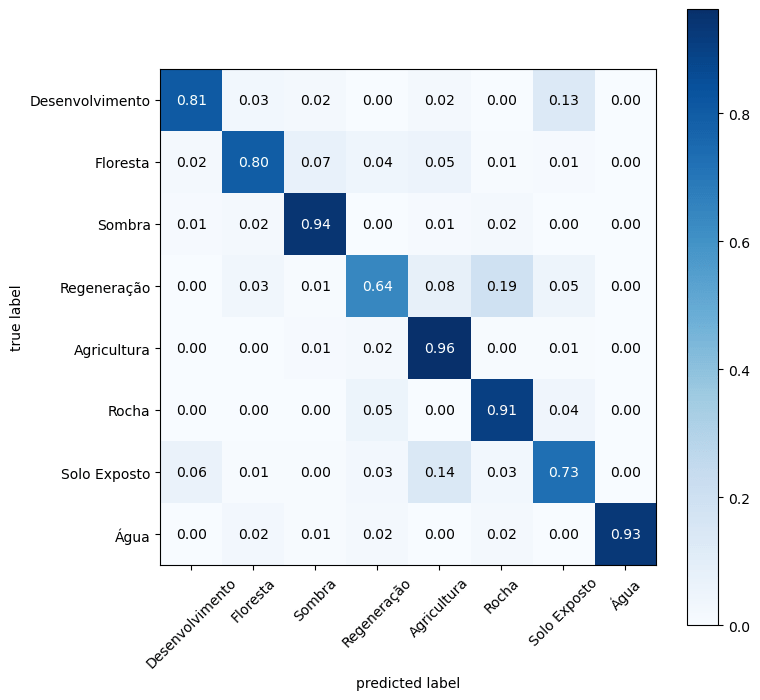
\includegraphics[width = 0.8\columnwidth]{./Figuras/cm/cm_cenario_31-min.png}}%% Modo apresentação: tamanho da figura
\mode<article>{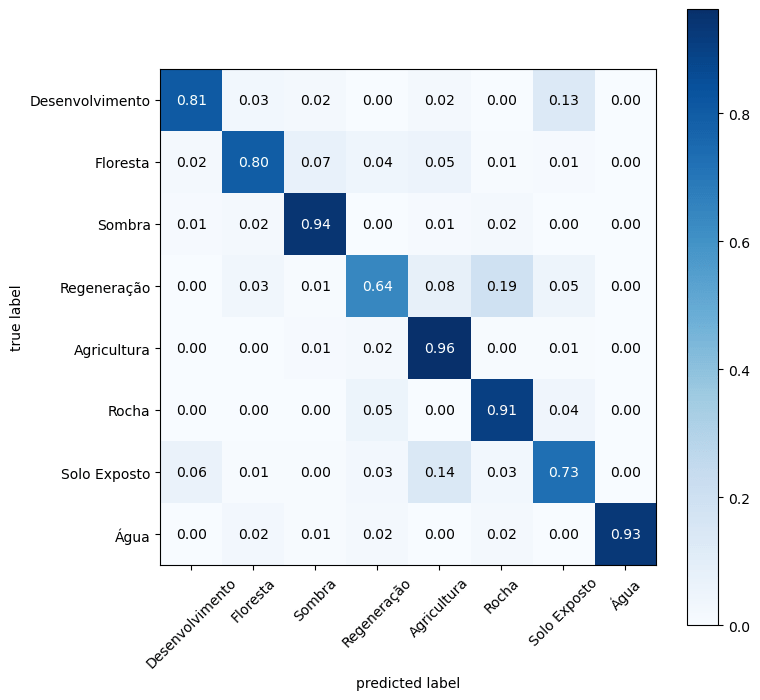
\includegraphics[width = 0.5\columnwidth]{./Figuras/cm/cm_cenario_31-min.png}}%% Modo artigo: tamanho da figura
\source{Autoria própria.}
\end{figure}

\column{0.5\linewidth}

\begin{figure}[!htb]
\centering%
\caption{Matriz de confusão do cenário 3 sem aumento de dados.}%
\label{fig:matriz:cen32}
\mode<presentation>{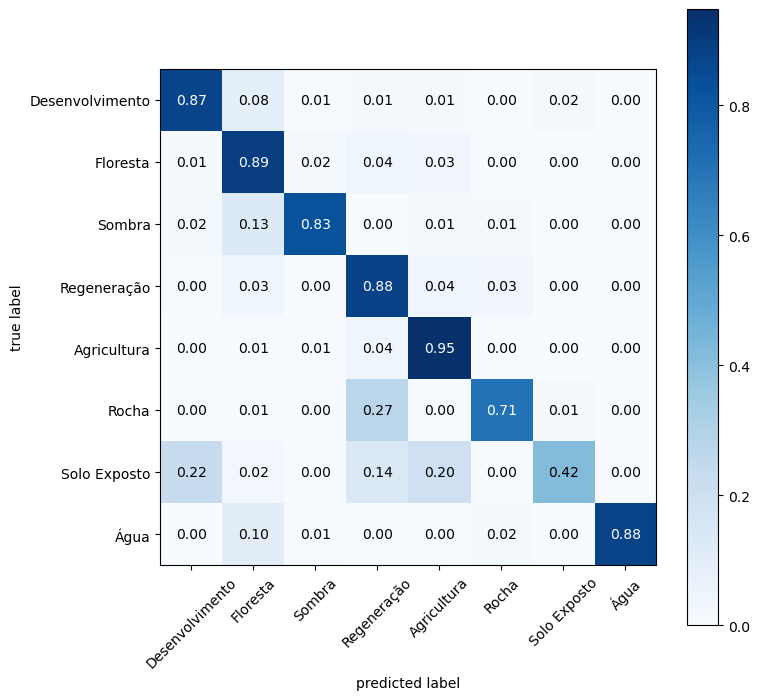
\includegraphics[width = 0.8\columnwidth]{./Figuras/cm/cm_cenario_32-min.png}}%% Modo apresentação: tamanho da figura
\mode<article>{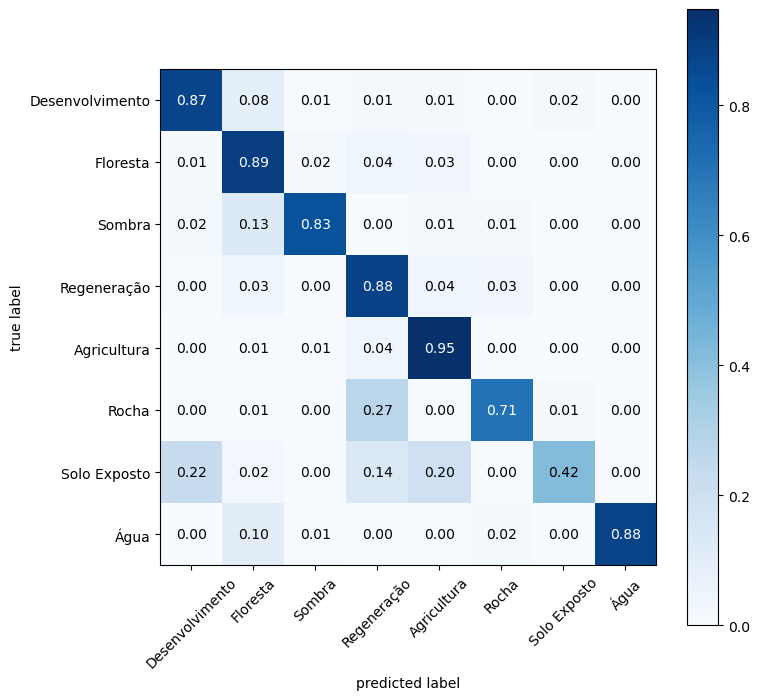
\includegraphics[width = 0.5\columnwidth]{./Figuras/cm/cm_cenario_32-min.png}}%% Modo artigo: tamanho da figura
\source{Autoria própria.}
\end{figure}

\end{columns}
\end{frame}

\begin{frame}

    \begin{itemize}
        \item \textcolor{lightgray}{\textbf{Cenário 1}: SegNet Modificada, usando a função de custo \textbf{Entropia Cruzada}.}
        \begin{itemize}
            \item \textcolor{lightgray}{Experimento 1: \textbf{pesos iguais (1)}.}
            \item \textcolor{lightgray}{Experimento 2: \textbf{pesos ponderados}.}
            \item \textcolor{lightgray}{Utilização de 9 classes (8 classes + \colorbox{yellow}{piscina}).}
        \end{itemize}
    \end{itemize}
    \begin{itemize}
        \item \textcolor{lightgray}{\textbf{Cenário 2}: SegNet Modificada, usando a função de custo \textbf{Entropia Cruzada}.}
        \begin{itemize}
            \item \textcolor{lightgray}{Experimento 1: \textbf{com aumento de dados}.}
            \item \textcolor{lightgray}{Experimento 2: \textbf{sem aumento de dados}.}
            \item \textcolor{lightgray}{Ambos usam pesos ponderados na função de custo.}
        \end{itemize}
    \end{itemize}
    \begin{itemize}
        \item \textcolor{lightgray}{\textbf{Cenário 3}: U-NET, usando a função de custo \textbf{Entropia Cruzada} com pesos ponderados.}
        \begin{itemize}
            \item \textcolor{lightgray}{Experimento 1: \textbf{com aumento de dados}.}
            \item \textcolor{lightgray}{Experimento 2: \textbf{sem aumento de dados}.}
        \end{itemize}
    \end{itemize}
    \begin{itemize}
        \item \textbf{Cenário 4}: SegNet Modificada e U-NET, usando a função de custo \textbf{Focal Loss}.
        \begin{itemize}
            \item Experimento 1: SegNet Modificada \textbf{com aumento de dados}.
            \item Experimento 2: U-NET \textbf{com aumento de dados}.
        \end{itemize}
    \end{itemize}
    
    % \begin{block}{Observações}
    %     Aumento de dados: \textbf{Espelhamento horizontal e vertical}.
    % \end{block}
\end{frame}

\begin{frame}
\framesubtitle{Cenário 4 - Análise dos Resultados}

\begin{columns}[T]

\column{0.5\linewidth}
\begin{table}[!ht]
    \centering
    \mode<presentation>{\scriptsize}%% Modo apresentação: tamanho de fonte
    \mode<article>{\small}%% Modo artigo: tamanho de fonte
    \caption{Resultados da SegNet no cenário 4 com \textit{Focal Loss}.}%% Legenda
    \label{tab:res:cen41}%% Rótulo
    \begin{tabular}{lllll}
    \toprule
        \textbf{Classe} & \textbf{Prec} & \textbf{Sens} & \textbf{F1-Score} & \textbf{IoU} \\
        \midrule
        \textbf{Desenvolvida}   & 0.85 & 0.86 & 0.86 & 0.75  \\ 
        \textbf{Floresta}       & 0.89 & 0.90 & 0.89 & 0.81  \\ 
        \textbf{Sombra}         & 0.89 & 0.74 & 0.81 & 0.68  \\ 
        \textbf{Regeneração}    & 0.75 & 0.89 & 0.81 & 0.68  \\ 
        \textbf{Agricultura}    & 0.85 & 0.85 & 0.85 & 0.74  \\ 
        \textbf{Rocha}          & 0.61 & 0.53 & 0.57 & 0.40  \\ 
        \textbf{Solo Exposto}   & 0.52 & 0.22 & 0.31 & 0.18  \\ 
        \textbf{Água}           & 0.98 & 0.43 & 0.60 & 0.42 \\ 
        \textbf{} & ~ & ~ & ~ & ~ \\ 
        \textbf{Acurácia} & 0.83 & ~ & \textbf{IoU} & 0.58 \\
        \bottomrule
        \addlinespace
    \end{tabular}
    \source{Autoria própria.}%% Fonte
\end{table}

\column{0.5\linewidth}

\begin{table}[!ht]
    \centering
    \mode<presentation>{\scriptsize}%% Modo apresentação: tamanho de fonte
    \mode<article>{\small}%% Modo artigo: tamanho de fonte
    \caption{Resultados da U-NET no cenário 4 com \textit{Focal Loss}.}%% Legenda
    \label{tab:res:cen42}%% Rótulo
    \begin{tabular}{lllll}
    \toprule
        \textbf{Classe} & \textbf{Prec} & \textbf{Sens} & \textbf{F1-Score} & \textbf{IoU} \\
        \midrule
        \textbf{Desenvolvida}    & \textbf{0.90} & \textbf{0.86} & \textbf{0.88} & \textbf{0.79}  \\ 
        \textbf{Floresta}        & \textbf{0.91} & \textbf{0.91} & \textbf{0.91} & \textbf{0.83}  \\ 
        \textbf{Sombra}          & \textbf{0.89} & \textbf{0.80} & \textbf{0.84} & \textbf{0.73}  \\ 
        \textbf{Regeneração}     & \textbf{0.80} & 0.88 & \textbf{0.84} & \textbf{0.72}  \\ 
        \textbf{Agricultura}     & \textbf{0.85} & \textbf{0.94} & \textbf{0.89} & \textbf{0.81}  \\ 
        \textbf{Rocha}           & \textbf{0.81} & \textbf{0.67} & \textbf{0.74} & \textbf{0.58}  \\ 
        \textbf{Solo Exposto}    & \colorbox{green!25}{0.75} & \textbf{0.36} & \colorbox{green!25}{0.49} & \colorbox{green!25}{0.32}  \\ 
        \textbf{Água}            & \textbf{0.99} & \colorbox{green!25}{0.89} & \colorbox{green!25}{0.94} & \colorbox{green!25}{0.88}  \\ 
        \textbf{} & ~ & ~ & ~ & ~ \\ 
        \textbf{Acurácia} & \colorbox{green!25}{0.87} & ~ & \textbf{IoU} & \colorbox{green!25}{0.71} \\
        \bottomrule
        \addlinespace
    \end{tabular}
    \source{Autoria própria.}%% Fonte
\end{table}

\end{columns}
\end{frame}

\begin{frame}
\framesubtitle{Cenário 4 - Matriz de Confusão}

\begin{columns}[T]

\column{0.5\linewidth}
\begin{figure}[!htb]
\centering%
\caption{Matriz de confusão do cenário 4 com \textit{Focal Loss}.}%
\label{fig:matriz:cen41}
\mode<presentation>{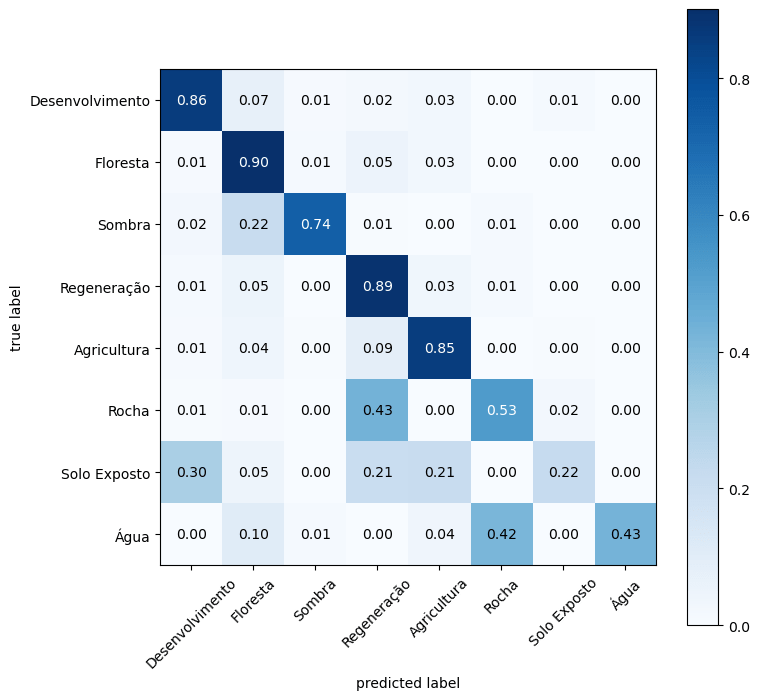
\includegraphics[width = 0.8\columnwidth]{./Figuras/cm/cm_cenario_41-min.png}}%% Modo apresentação: tamanho da figura
\mode<article>{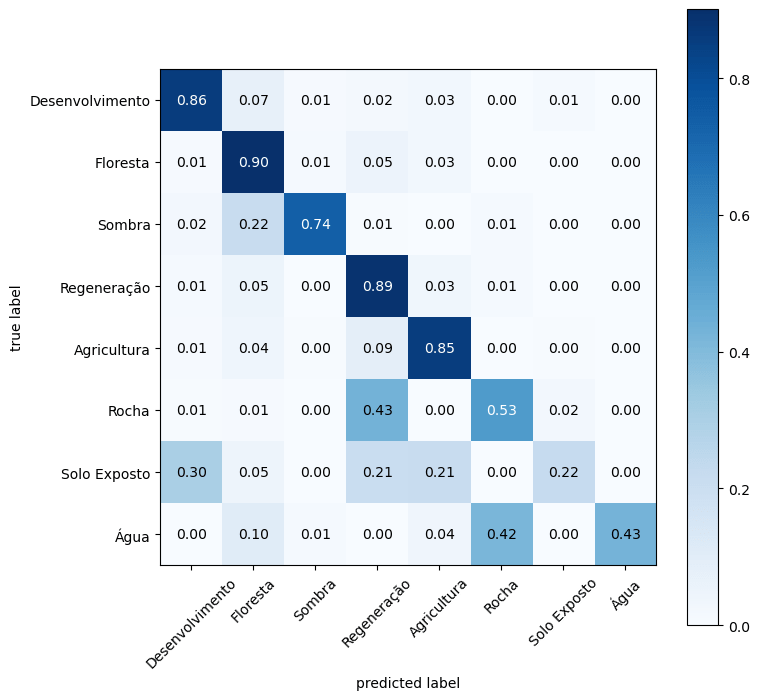
\includegraphics[width = 0.5\columnwidth]{./Figuras/cm/cm_cenario_41-min.png}}%% Modo artigo: tamanho da figura
\source{Autoria própria.}
\end{figure}

\column{0.5\linewidth}

\begin{figure}[!htb]
\centering%
\caption{Matriz de confusão do cenário 4 com \textit{Focal Loss}.}%
\label{fig:matriz:cen42}
\mode<presentation>{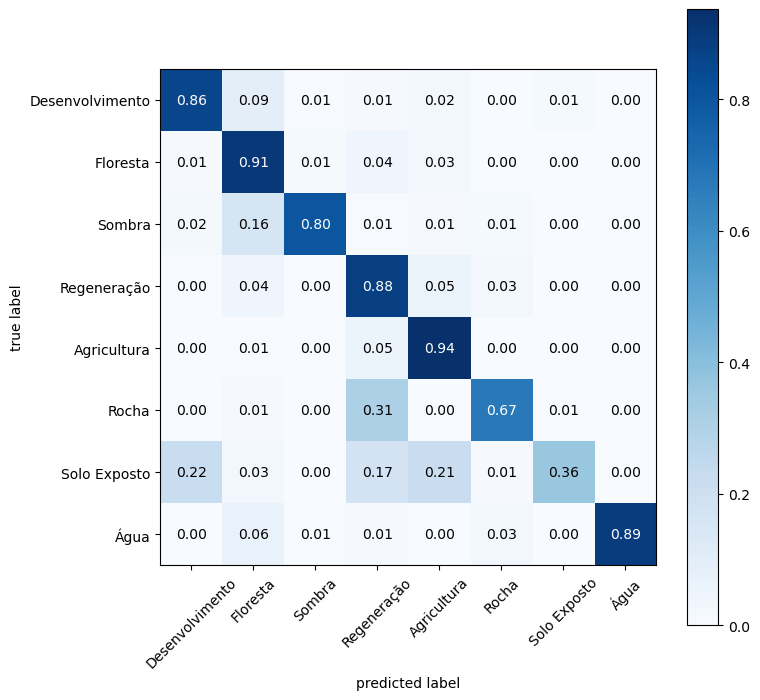
\includegraphics[width = 0.8\columnwidth]{./Figuras/cm/cm_cenario_42-min.png}}%% Modo apresentação: tamanho da figura
\mode<article>{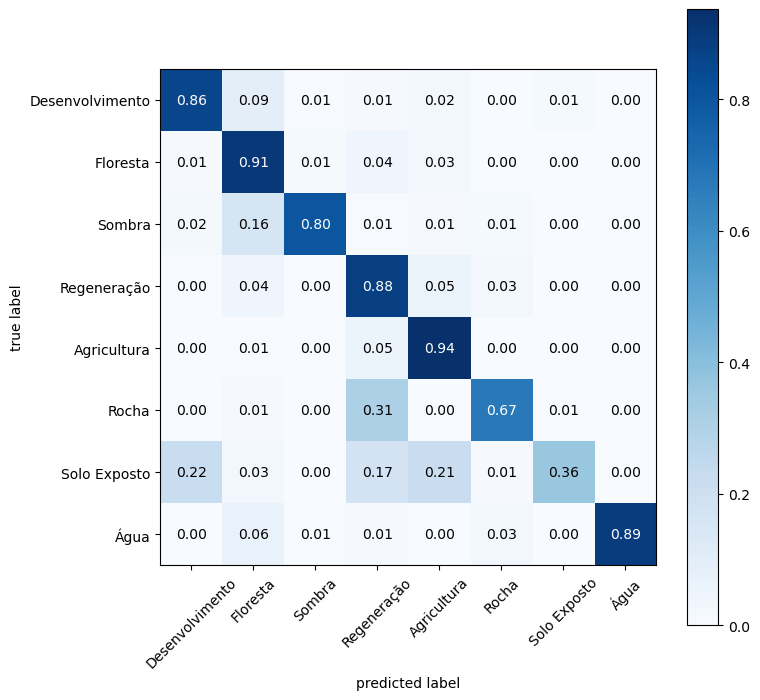
\includegraphics[width = 0.5\columnwidth]{./Figuras/cm/cm_cenario_42-min.png}}%% Modo artigo: tamanho da figura
\source{Autoria própria.}
\end{figure}

\end{columns}
\end{frame}

\begin{frame}
\framesubtitle{Comparação dos Resultados - Acurácia}

\begin{table}[!ht]
    \centering
    \mode<presentation>{\scriptsize}%% Modo apresentação: tamanho de fonte
    \mode<article>{\small}%% Modo artigo: tamanho de fonte
    \caption{Comparativo de acurária dos experimentos em cada cenário.}%% Legenda
    \label{tab:res:acuracia}%% Rótulo
    \begin{tabular}{lrrrr}
    \toprule
        \textbf{} & \textbf{Cenário 1} & \textbf{Cenário 2} & \textbf{Cenário 3} & \textbf{Cenário 4} \\
        \midrule
        \textbf{Experimento 01}  & 0.81 & 0.76 & 0.81 & 0.83 \\ 
        \textbf{Experimento 02}  & 0.65 & 0.79 & \colorbox{green!25}{0.87}\footnote{U-NET com função de custo de entropia cruzada e pesos ponderados. Sem aumento de dados} & \colorbox{green!25}{0.87}\footnote{U-NET com função de custo \textit{Focal Loss}. Com aumento de dados} \\
        \bottomrule
        \addlinespace
    \end{tabular}
    \source{Autoria própria.}%% Fonte
\end{table}

\textcolor{gray!25}{
\begin{table}[!ht]
    \centering
    \mode<presentation>{\scriptsize}%% Modo apresentação: tamanho de fonte
    \mode<article>{\small}%% Modo artigo: tamanho de fonte
    % \caption{Comparativo de IoU dos experimentos em cada cenário.}%% Legenda
    % \label{tab:res:iou}%% Rótulo
    \begin{tabular}{lrrrr}
    \toprule
        \textbf{} & \textbf{Cenário 1} & \textbf{Cenário 2} & \textbf{Cenário 3} & \textbf{Cenário 4} \\
        \midrule
        \textbf{Experimento 01}  & 0.48 & 0.40 & 0.65 & 0.58 \\ 
        \textbf{Experimento 02}  & 0.40 & 0.62 & \colorbox{green!25}{0.72} & \colorbox{green!25}{0.71} \\
        \bottomrule
        \addlinespace
    \end{tabular}
    \source{Autoria própria.}%% Fonte
\end{table}}

\end{frame}

\begin{frame}
    \setcounter{footnote}{0}
    \framesubtitle{Comparação dos Resultados - IoU}
    
    \textcolor{gray!25}{
    \begin{table}[!ht]
        \centering
        \mode<presentation>{\scriptsize}%% Modo apresentação: tamanho de fonte
        \mode<article>{\small}%% Modo artigo: tamanho de fonte
        % \caption{Comparativo de acurária dos experimentos em cada cenário.}%% Legenda
        % \label{tab:res:acuracia}%% Rótulo
        \begin{tabular}{lrrrr}
        \toprule
            \textbf{} & \textbf{Cenário 1} & \textbf{Cenário 2} & \textbf{Cenário 3} & \textbf{Cenário 4} \\
            \midrule
            \textbf{Experimento 01}  & 0.81 & 0.76 & 0.81 & 0.83 \\ 
            \textbf{Experimento 02}  & 0.65 & 0.79 & \colorbox{green!25}{0.87} & \colorbox{green!25}{0.87} \\
            \bottomrule
            \addlinespace
        \end{tabular}
        \source{Autoria própria.}%% Fonte
    \end{table}}
    
    \begin{table}[!ht]
        \centering
        \mode<presentation>{\scriptsize}%% Modo apresentação: tamanho de fonte
        \mode<article>{\small}%% Modo artigo: tamanho de fonte
        \caption{Comparativo de IoU dos experimentos em cada cenário.}%% Legenda
        \label{tab:res:iou}%% Rótulo
        \begin{tabular}{lrrrr}
        \toprule
            \textbf{} & \textbf{Cenário 1} & \textbf{Cenário 2} & \textbf{Cenário 3} & \textbf{Cenário 4} \\
            \midrule
            \textbf{Experimento 01}  & 0.48 & 0.40 & 0.65 & 0.58 \\ 
            \textbf{Experimento 02}  & 0.40 & 0.62 & \colorbox{green!25}{0.72}\footnote{U-NET com função de custo de entropia cruzada e pesos ponderados. Sem aumento de dados} & \colorbox{green!25}{0.71}\footnote{U-NET com função de custo \textit{Focal Loss}. Com aumento de dados} \\
            \bottomrule
            \addlinespace
        \end{tabular}
        \source{Autoria própria.}%% Fonte
    \end{table}
    
\end{frame}

\begin{frame}
\setcounter{footnote}{0}
\framesubtitle{Comparação dos Resultados - Medida $f$}

\begin{table}[!ht]
    \caption{Resultados da medida $f$ dos experimentos nos melhores cenários}%% Legenda
    \centering
    \begin{tabular}{lllll}
    \toprule
        \multirow{2}{*}{\textbf{Classe}} & \multicolumn{2}{c}{\textbf{Cenário 3}} & \multicolumn{2}{c}{\textbf{Cenário 4}} \\ 
        \cline{2-5} & Exp 1 & Exp 2\footnote{U-NET com função de custo de entropia cruzada e pesos ponderados. Sem aumento de dados} & Exp 1 & Exp 2\footnote{U-NET com função de custo \textit{Focal Loss}. Com aumento de dados} \\
        \midrule
        \textbf{Área Desenvolvida}          & 0.85 & \colorbox{green!25}{0.88} & 0.86 & \colorbox{green!25}{0.88} \\
        \textbf{Floresta}                   & 0.87 & \colorbox{green!25}{0.91} & 0.89 & \colorbox{green!25}{0.91} \\
        \textbf{Sombra}                     & 0.79 & \colorbox{green!25}{0.85} & 0.81 & \colorbox{green!25}{0.84} \\
        \textbf{Área em Regeneração}        & 0.73 & \colorbox{green!25}{0.85} & 0.81 & \colorbox{green!25}{0.84} \\
        \textbf{Agricultura}                & 0.87 & \colorbox{green!25}{0.90} & 0.85 & \colorbox{green!25}{0.89} \\
        \textbf{Rocha}                      & 0.66 & \colorbox{green!25}{0.75} & 0.57 & \colorbox{green!25}{0.74} \\
        \textbf{Solo Exposto}               & 0.43 & \colorbox{green!25}{0.52} & 0.31 & \colorbox{green!25}{0.49} \\
        \textbf{Água}                       & \colorbox{green!25}{0.95} & 0.93 & 0.60 & \colorbox{green!25}{0.94} \\ 
        \bottomrule
        \addlinespace
    \end{tabular}
    \label{tab:res:fscore:classe}%% Rótulo
    \source{Autoria própria.}%% Fonte
\end{table}

\end{frame}

\begin{frame}
    \setcounter{footnote}{0}
    \framesubtitle{Comparação dos Resultados - Medida $IoU$}
    
    \begin{table}[!ht]
        \caption{Resultados da medida $IoU$ dos experimentos nos melhores cenários}%% Legenda
        \centering
        \begin{tabular}{lllll}
        \toprule
            \multirow{2}{*}{\textbf{Classe}} & \multicolumn{2}{c}{\textbf{Cenário 3}} & \multicolumn{2}{c}{\textbf{Cenário 4}} \\ 
            \cline{2-5} & Exp 1 & Exp 2\footnote{U-NET com função de custo de entropia cruzada e pesos ponderados. Sem aumento de dados} & Exp 1 & Exp 2\footnote{U-NET com função de custo \textit{Focal Loss}. Com aumento de dados} \\
            \midrule
            \textbf{Área Desenvolvida}          & 0.73 & \colorbox{green!25}{0.79} & 0.75 & \colorbox{green!25}{0.79} \\ 
            \textbf{Floresta}                   & 0.77 & \colorbox{green!25}{0.83} & 0.81 & \colorbox{green!25}{0.83} \\ 
            \textbf{Sombra}                     & 0.65 & \colorbox{green!25}{0.73} & 0.68 & \colorbox{green!25}{0.73} \\ 
            \textbf{Área em Regeneração}        & 0.58 & \colorbox{green!25}{0.74} & 0.68 & \colorbox{green!25}{0.72} \\ 
            \textbf{Agricultura}                & 0.77 & \colorbox{green!25}{0.82} & 0.74 & \colorbox{green!25}{0.81} \\ 
            \textbf{Rocha}                      & 0.49 & \colorbox{green!25}{0.60} & 0.40 & \colorbox{green!25}{0.58} \\ 
            \textbf{Solo Exposto}               & 0.28 & \colorbox{green!25}{0.35} & 0.18 & \colorbox{green!25}{0.32} \\ 
            \textbf{Água}                       & \colorbox{green!25}{0.90} & 0.86 & 0.42 & \colorbox{green!25}{0.88} \\ 
            \bottomrule
            \addlinespace
        \end{tabular}
        \label{tab:res:iou:classe}%% Rótulo
        \source{Autoria própria.}%% Fonte
    \end{table}
    
\end{frame}

\begin{frame}
\framesubtitle{Comparação dos Resultados - Análise Visual}

\begin{figure}[htp]%% Ambiente figure
    \centering
    \parbox{6cm}{
        \mode<presentation>{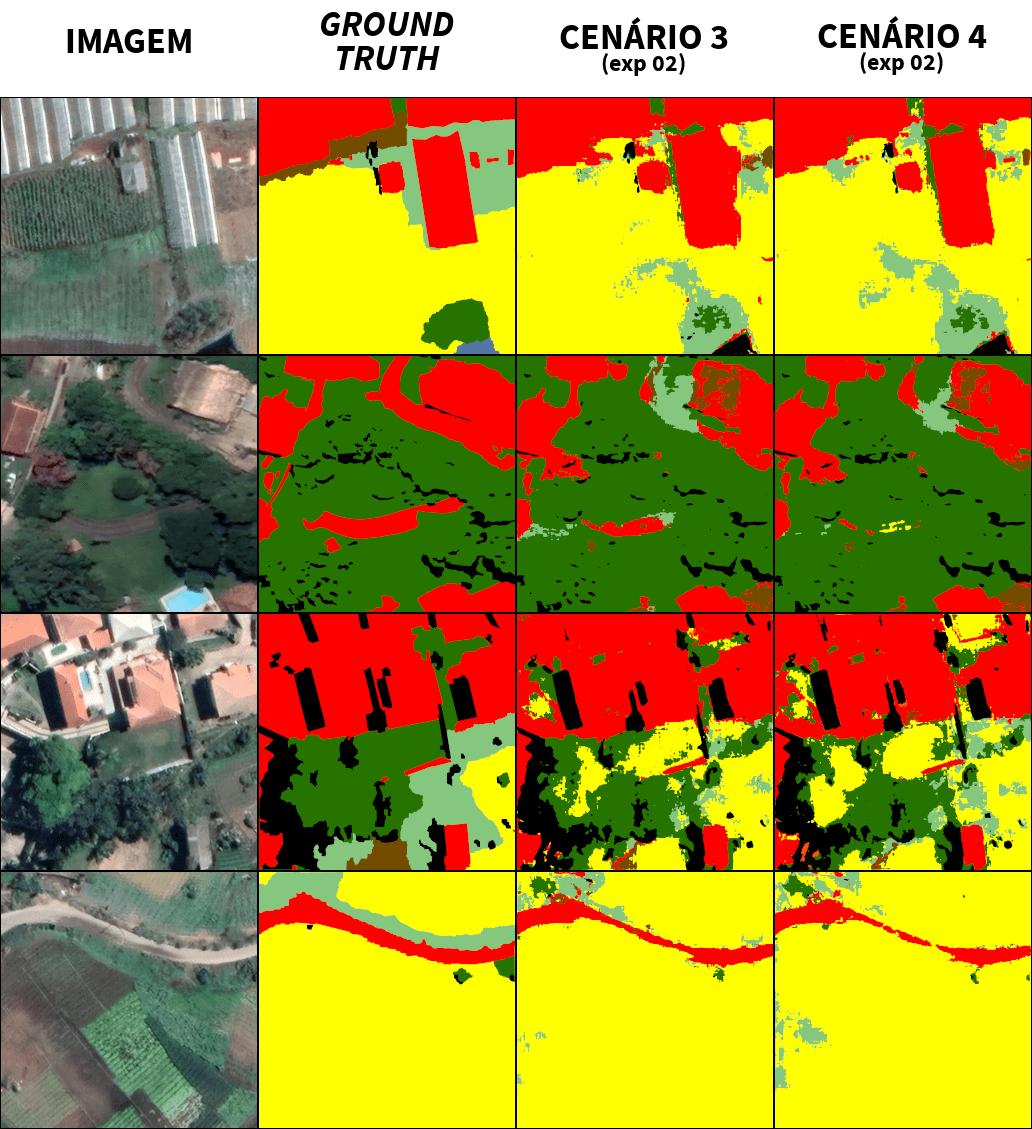
\includegraphics[width = 5cm]{./Figuras/cm/comparativo_01-min}}%% Modo apresentação: tamanho da figura
        \mode<article>{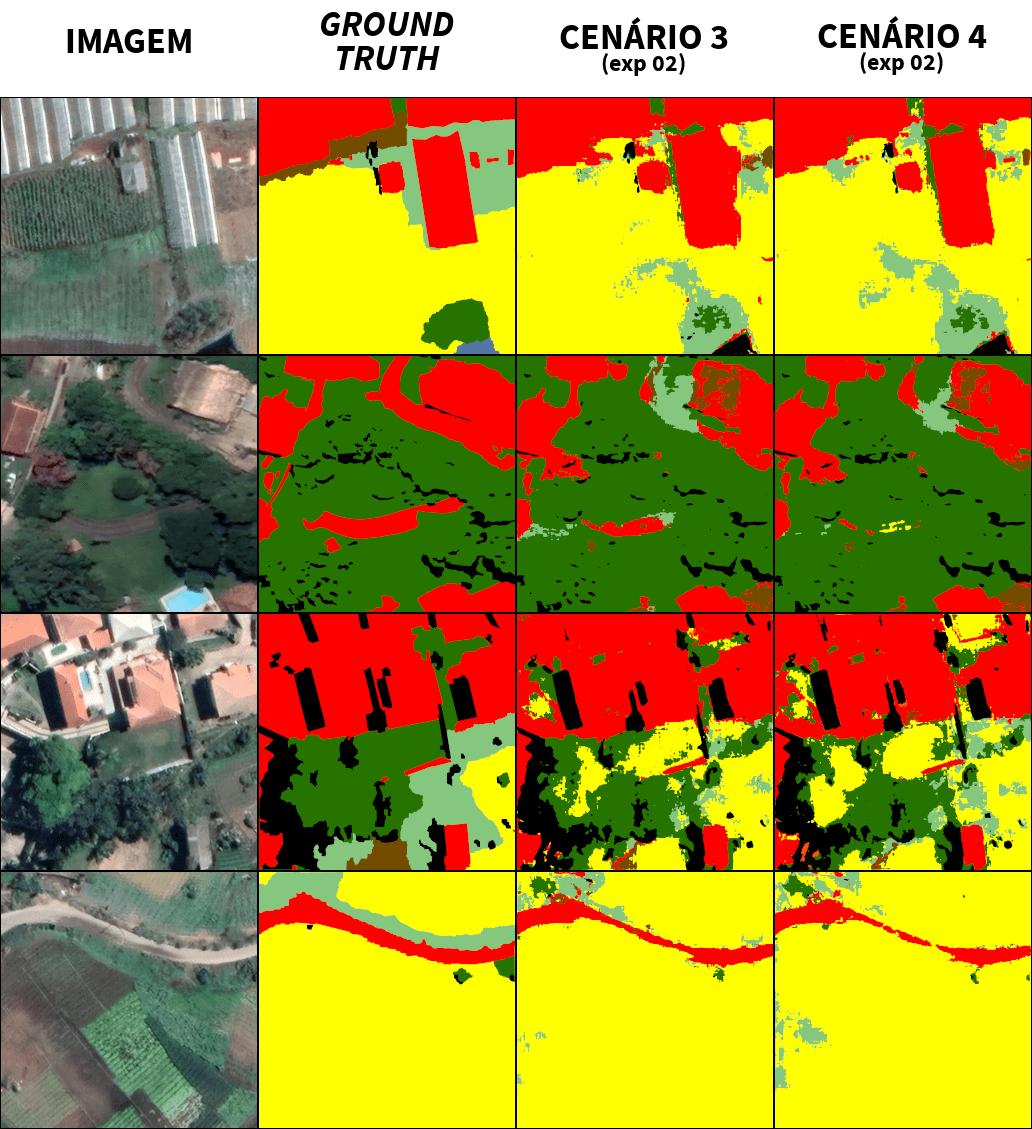
\includegraphics[width = 0.2\columnwidth]{./Figuras/cm/comparativo_01-min}}%% Modo artigo: tamanho da figura
        \caption{Comparativo entre as Imagens do Conjunto de Teste}
        \label{fig:res:comparativo1}}
    \qquad
        \begin{minipage}{6cm}
            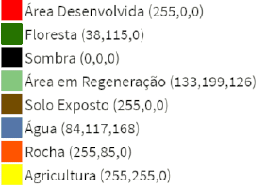
\includegraphics[width=4cm]{Figuras/legenda}
            \caption{Legenda}
            \label{fig:res:legenda1}
        \end{minipage}
    \source{Autoria própria.}%% Fonte
\end{figure}

\end{frame}

\begin{frame}
    \framesubtitle{Comparação dos Resultados - Análise Visual}
    
    \begin{figure}[htp]%% Ambiente figure
        \centering
        \parbox{6cm}{
            \mode<presentation>{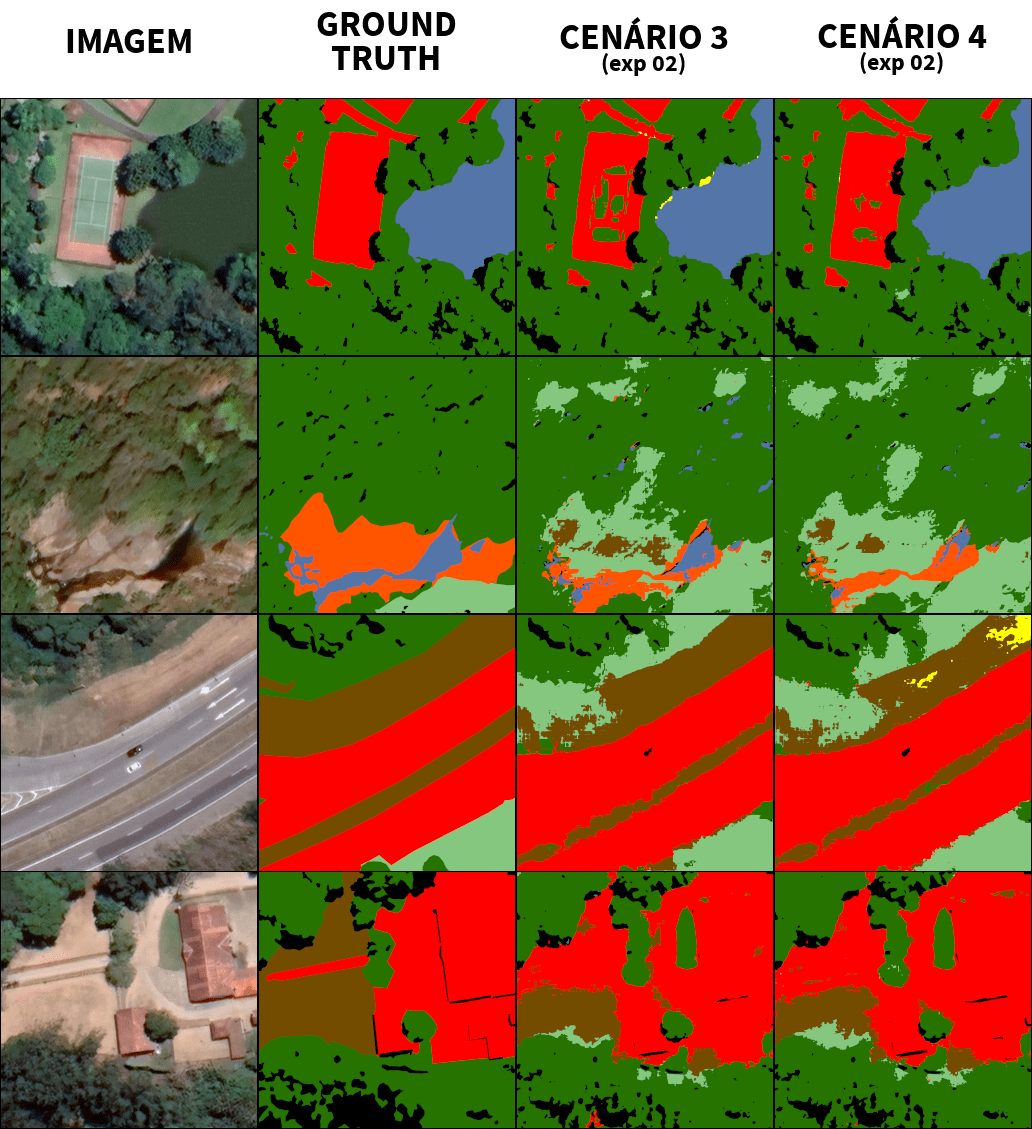
\includegraphics[width=5cm]{./Figuras/cm/comparativo_02-min}}%% Modo apresentação: tamanho da figura
        \mode<article>{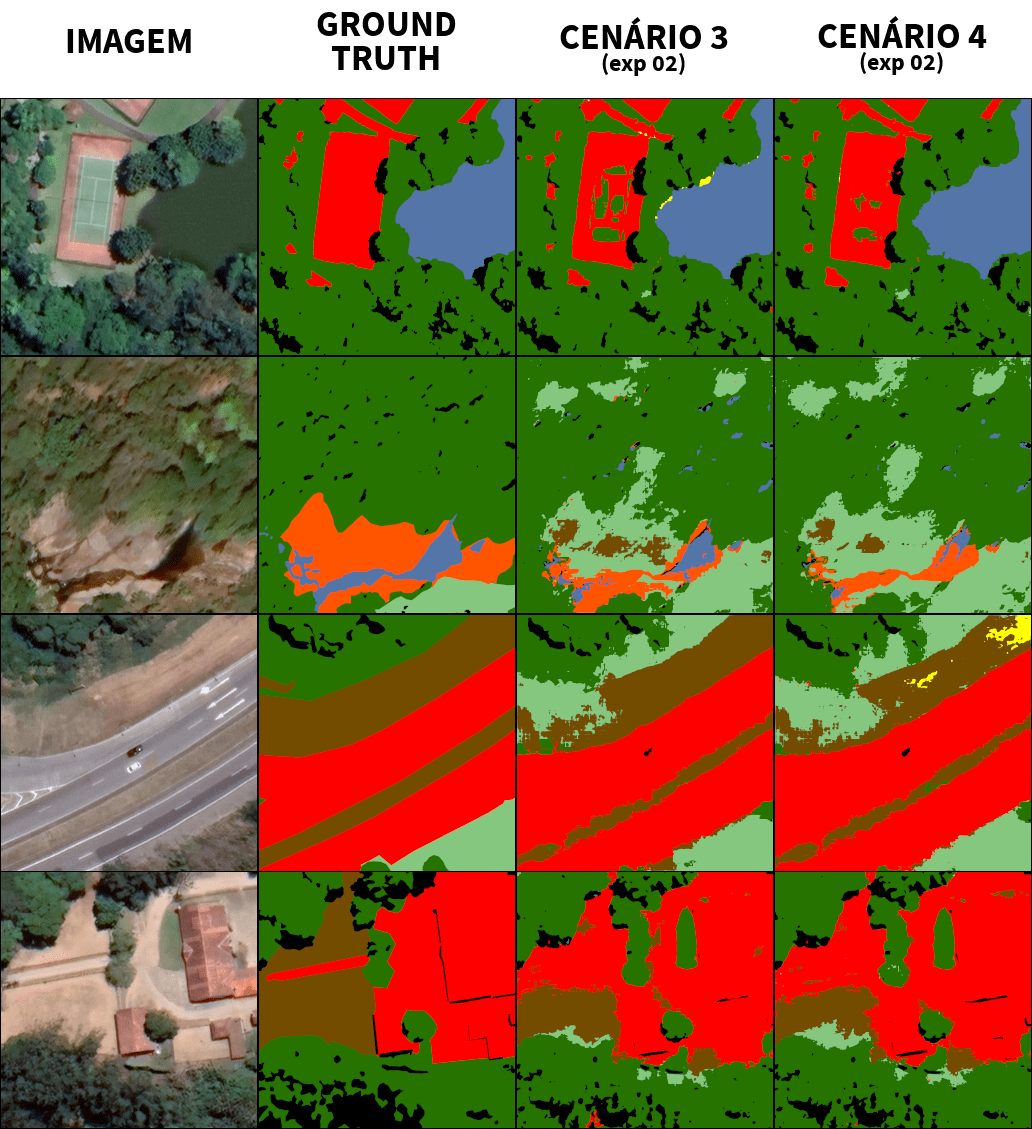
\includegraphics[width = 0.2\columnwidth]{./Figuras/cm/comparativo_02-min}}%% Modo artigo: tamanho da figura
            \caption{Comparativo entre as Imagens do Conjunto de Teste}
            \label{fig:res:comparativo2}}
        \qquad
            \begin{minipage}{6cm}
                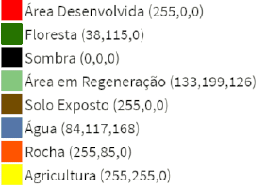
\includegraphics[width=4cm]{Figuras/legenda}
                \caption{Legenda}
                \label{fig:res:legenda2}
            \end{minipage}
        \source{Autoria própria.}%% Fonte
    \end{figure}
    
\end{frame}

\begin{frame}
\framesubtitle{Comparação com trabalhos relacionados}
\begin{columns}[T]

\column{0.5\linewidth}
    \begin{figure}[!htb]
        \centering%
        \caption{Resultado da segmentação semântica no conjunto de dados do Google com a arquitetura proposta.}%
        \mode<presentation>{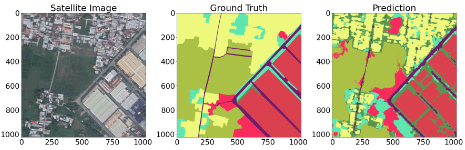
\includegraphics[width = 0.8\columnwidth]{./Figuras/khan-01}}%% Modo apresentação: tamanho da figura
        \mode<article>{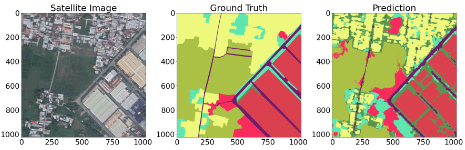
\includegraphics[width = 0.4\columnwidth]{./Figuras/khan-01}}%% Modo artigo: tamanho da figura
        \source{Adaptado de \cite{Khanh2021}.}
    \end{figure}

\column{0.5\linewidth}

    \begin{itemize}
        \item Arquitetura baseada na U-NET \textit{Encoder-Decoder}.
        \item Segmentação semântica usando imagens de satélite de alta resolução do Google Earth.
        \item Anotação manual com a ferramenta CVAT \cite{cvat}.
        \item Conjunto de dados com 12 classes.
        \item Comparação do resultado com diferentes funções de custo (EfficientNet-B0)
        \item Não apresentaram métricas de avaliação.
    \end{itemize}

\end{columns}
\end{frame}

\section{Conclusões}\label{sec:concl}

\subsection{Considerações finais}\label{ssec:concl1}

\begin{frame}
\begin{itemize}
    \item Propomos uma metodologia de baixo custo.
    \item Imagens RGB do Google Earth.
    \item Desempenho superior da U-NET em relação à SegNet Modificada.
    \item Tempo de treinamento e teste com a rede U-NET é menor que o da SegNet Modificada.
    \item Aumento de performance a cada novo cenário proposto.
    \item Junção da classe \textbf{Piscina} com a classe \textbf{Área Desenvolvida} a partir do cenário 2.
\end{itemize}
\end{frame}

\section{Conclusões}\label{sec:concl}

\subsection{Trabalhos futuros}\label{ssec:concl1}

\begin{frame}
\begin{itemize}
    \item Ampliar o conjunto de dados.
    \item Utilizar técnicas de pós-processamento para melhorar a segmentação.
    \item Contribuir no mapeamento do uso e cobertura da terra em áreas de proteção ambiental.
\end{itemize}
\end{frame}

\mode<presentation>{%% Modo apresentação: referências
  \section{\refname}\label{sec:refs}%
  \frame[allowframebreaks]{%
    \framesubtitle{~}%
    \printbibliography[heading = none]%
  }%
}

\mode<article>{\printbibliography}%% Modo artigo: referências

\section{Agradecimentos}\label{sec:agrad}

\begin{frame}{}{\mode<presentation>{~}}
    \begin{minipage}[c][\textheight][c]{\textwidth}
        \centering
        \title{REDES NEURAIS CONVOLUCIONAIS NA SEGMENTAÇÃO SEMÂNTICA DE IMAGENS AÉREAS PARA O MAPEAMENTO DA COBERTURA DA TERRA EM ÁREAS DE PROTEÇÃO AMBIENTAL}
        \author{Fabricio Bizotto}
        \date{\today}
        \maketitle
    \end{minipage}
\end{frame}

% \respnotice[Declaração de Responsabilidade]{O(s) autor(es) é(são) o(s) único(s) responsável(eis) pelas informações contidas neste documento.}

% \begin{frame}{}{\mode<presentation>{~}}
% Às organizações de fomento, pelo apoio recebido para o desenvolvimento deste trabalho e a participação neste evento:
% \begin{center}
% \includegraphics[height = 10mm]{./Logos/apoio-capes}
% \hfill%
% \includegraphics[height = 10mm]{./Logos/apoio-cnpq}
% \hfill%
% \includegraphics[height = 10mm]{./Logos/apoio-fa-gov-pr}
% \hfill%
% \includegraphics[height = 10mm]{./Logos/utfpr}
% \end{center}
% \mode<presentation>{%% Modo apresentação: agradecimentos e declaração de responsabilidade
%   Aos presentes, pela atenção\sfootnote[frame]{\faStickyNoteO~\textbf{\respnoticetitle:}\space\MakeLowercase{\respnoticetext}}.%
% }
% \end{frame}

% \mode<article>{%% Modo artigo: declaração de responsabilidade
%   \section{\respnoticetitle}\label{sec:declar}%
%   \respnoticetext%
% }

%% Fim do documento
\end{document}